% !TeX root = main.tex
% !TeX document-id = {c6282027-a510-40f1-b05e-2f558a6cd3f1}
% !TEX encoding = UTF-8 Unicode
% !TeX TXS-program:compile = txs:///xelatex/[--shell-escape]|txs:///bibtex|txs:///xelatex/[--shell-escape]|txs:///xelatex/[--shell-escape]
%%%%%%%%%%%%%%%%%%%%%%%%%%%%%%%%%%%%%%%%%%%%%%%%%%%%%%%%%%%%%%%%%%%%%%%%
% Plantilla TFG/TFM
% Universidad de Murcia. Facultad de Informática
% Realizado por: José Manuel Requena Plens
% Modificado: Pablo José Rocamora Zamora
% Contacto: pablojoserocamora@gmail.com
%%%%%%%%%%%%%%%%%%%%%%%%%%%%%%%%%%%%%%%%%%%%%%%%%%%%%%%%%%%%%%%%%%%%%%%%


% Archivo .TEX que incluye todas las configuraciones del documento y los paquetes. Añade todo aquello que necesites utilizar en el documento en este archivo.
% En él se encuentra la configuración de los márgenes, establecidos según las directrices de estilo de la EPS.
\input{include/configuracioninicial}

%%%%%%%%%%%%%%%%%%%%%%%%%%%%%%%%%%%%%%%%%%%%%%%%%%%%%%%%%%%%%%%%%%%%%%
% INFORMACIÓN DEL TFG
% Comentar lo que NO se desee añadir y sustituir con la información correcta.
%%%%%%%%%%%%%%%%%%%%%%%%%%%%%%%%%%%%%%%%%%%%%%%%%%%%%%%%%%%%%%%%%%%%%%
% Título y subtítulo
\newcommand{\titulo}{Mitigación de alucinaciones en LLMs mediante el desarrollo de un sistema RAG para la verificación de noticias}
\newcommand{\subtitulo}{Evaluación comparativa de recuperación léxica y semántica con modelos de lenguaje de distinta escala}
% Datos del autor
\newcommand{\miNombre}{Javier Ruiz Chicoy}
\newcommand{\miDNI}{49245871L}
\newcommand{\miEmail}{j.ruizchicoy@um.es}
% Datos del tutor/es
\newcommand{\miTutor}{Rafael Valencia García}
\newcommand{\miTutorB}{Ronghao Pan}
% Datos de la facultada y universidad
\newcommand{\miFacultad}{Facultad de Informática}
\newcommand{\miFacultadCorto}{FIUM}
\newcommand{\miUniversidad}{\protect{Universidad de Murcia}}
\newcommand{\miUbicacion}{Murcia}
\newcommand{\firma}{include/firma}

% Configuración automática según el identificador elegido
% Grados
\definecolor{informatica}{RGB}{0,113,206}
% Colores generales
\definecolor{negro}{RGB}{0,0,0}
\definecolor{blanco}{RGB}{255,255,255}

% Logotipos comunes de todas las titulaciones
\newcommand{\logoFacultadPortada}{include/logos-titulaciones/logo_facultad}
\newcommand{\logoGradoPortada}{include/logos-titulaciones/logo_facultad}
\newcommand{\logoUniversidadPortada}{include/logos-universidad/logo_universidad}
\newcommand{\logoFacultadPortadaBaja}{include/logos-titulaciones/logo_facultad_y_texto}
% Logos
\newcommand{\logoGrado}{include/logos-titulaciones/FI-positivo}
\newcommand{\logoDepartamento}{include/logos-titulaciones/Logotipo_DIIC}
\newcommand{\logoUniversidad}{include/logos-universidad/um}
% Texto
\newcommand{\miGrado}{Grado en Ciencia e Ingeniería de Datos}
\newcommand{\tipotrabajo}{Trabajo Fin de Grado}
% Color
\newcommand{\colorgrado}{informatica}
\newcommand{\colortexto}{blanco}

% Información añadida a las propiedades del archivo PDF.
\hypersetup{
	pdfauthor = {\miNombre~(\miEmail)},
	pdftitle = {\titulo},
}

%%
% Archivo de acrónimos
%%
\makeglossaries % Genera la base de datos de acrónimos
\input{anexos/_acronimos.tex} % Archivo que contiene los acrónimos

%%%%%%%%%%%%%%%%%%%%%%%% 
% INICIO DEL DOCUMENTO
% A partir de aquí debes empezar a realizar tu TFG/TFM
%%%%%%%%%%%%%%%%%%%%%%%%
\begin{document}
	
	% Números romanos hasta el mainmatter.
	\frontmatter
	
	% PORTADA
	\input{include/portada/portada_color} % Portada Color
	\input{include/portada/portada_bn} % Portada B/N
	
	%%%%% PREAMBULO
	% Incluye el .tex que contiene el preámbulo, agradecimientos y dedicatorias.
	%\setstretch{1.5} % 1.5 línea de interlineado antes esta a 1 para la portada
	%%%%%%%%%%%%%%%%%%%%%%%%%%%%%%%%%%%%%%%%%%%%%%%%%%%%%%%%%%%%%%%%%%%%%%%%
% Plantilla TFG/TFM
% Universidad de Murcia. Facultad de Informática
% Realizado por: José Manuel Requena Plens
% Modificado: Pablo José Rocamora Zamora
% Contacto: pablojoserocamora@gmail.com
%%%%%%%%%%%%%%%%%%%%%%%%%%%%%%%%%%%%%%%%%%%%%%%%%%%%%%%%%%%%%%%%%%%%%%%%


\chapter*{Preámbulo}
\thispagestyle{empty}

El avance de los LLMs ha transformado profundamente la manera en que accedemos y generamos información. Sin embargo, esta misma capacidad los convierte en una herramienta potencialmente peligrosa en un ecosistema mediático donde la desinformación se propaga a una velocidad que los mecanismos de verificación tradicionales son incapaces de absorber.

Este Trabajo Fin de Grado nace del pensamiento de que la tecnología que forma parte del problema puede también ser parte de la solución. A lo largo de estas páginas se describe el diseño, implementación y validación de un sistema de \textit{Fact-Checking} automatizado construido sobre una arquitectura de Generación Aumentada por Recuperación (RAG), con el objetivo de mitigar las alucinaciones de los modelos de lenguaje anclando sus respuestas en un corpus real de noticias.

\cleardoublepage %salta a nueva página impar

\chapter*{Agradecimientos}

\thispagestyle{empty}
\vspace{1cm}

En primer lugar, quiero expresar mi más sincero agradecimiento a mis tutores, cuya ayuda me ha ayudado a ir mucho más allá de lo que tenía previsto cuando empecé con este TFG. Sin su implicación, muchas de las decisiones técnicas que sustentan esta memoria no habrían madurado de la misma manera.

A mis padres, María José e Isidoro, no tengo palabras suficientes para agradeceros todo lo que habéis hecho por mí. Habéis sido el pilar sobre el que se ha sostenido no solo estos 4 años, sino cada etapa de mi vida. Gracias por haberme dado la oportunidad de estudiar lo que me gusta y por estar siempre ahí, sin condiciones y sin importar el momento.

A mi pareja Laura, gracias por aguantarme en los momentos de más estrés, hacerme ver lo mejor de mí y por no quejarte demasiado cuando he tenido la cabeza en otro sitio. Tu apoyo ha sido mucho más importante de lo que probablemente imaginas, y este trabajo al igual que cada logro que consigo también es un poco tuyo.

A mis abuelas y abuelos, por el cariño y el apoyo que han transmitido y transmiten con cada conversación, y por el orgullo que sienten de manera incondicional en todo lo que hago. Sois mi mayor ejemplo de perseverancia, solidaridad y amor. Por eso, y por todo lo que me habéis dado, gracias.

A mis amigos Antonio, Juanjo, Javi y Álvaro, que he conocido por el camino. En vosotros he encontrado a una familia con la que compartir no solo esta etapa, sino también muchas más que vendrán después. Gracias por los momentos de risas, las conversaciones y por hacer de la universidad un lugar que siempre recordaré.

Por último, a todas las personas que de una forma u otra han estado ahí durante este proceso: gracias. Saber que contaba con vosotros ha hecho que todo fuera mucho más llevadero.

\cleardoublepage %salta a nueva página impar

% Aquí va la dedicatoria si la hubiese. Si no, comentar la(s) linea(s) siguientes
%\chapter*{}
%\setlength{\leftmargin}{0.5\textwidth}
%\setlength{\parsep}{0cm}
%\addtolength{\topsep}{0.5cm}
%
%\begin{flushright}
%	\small\em{
%		A mis padres, María José e Isidoro, y a Laura.\\
%		Por todo lo que hay detrás de estas páginas.
%	}
%\end{flushright}


\cleardoublepage %salta a nueva página impar

% Aquí va la cita célebre si la hubiese. Si no, comentar la(s) linea(s) siguientes
\chapter*{}

\setlength{\leftmargin}{0.5\textwidth}
\setlength{\parsep}{0cm}
\addtolength{\topsep}{0.5cm}
\begin{flushright}
	\small\em{
		Buscando el bien de nuestros semejantes,\\
		encontramos el nuestro
	}
\end{flushright}

\begin{flushright}
	\small{
		Platon.
	}
\end{flushright}

\cleardoublepage %salta a nueva página impar


	\input{preambulos/1_declaracion_originalidad}
	%%%%%%%%%%%%%%%%%%%%%%%%%%%%%%%%%%%%%%%%%%%%%%%%%%%%%%%%%%%%%%%%%%%%%%%%
% Plantilla TFG/TFM
% Universidad de Murcia. Facultad de Informática
% Realizado por: José Manuel Requena Plens
% Modificado: Pablo José Rocamora Zamora
% Contacto: pablojoserocamora@gmail.com
%%%%%%%%%%%%%%%%%%%%%%%%%%%%%%%%%%%%%%%%%%%%%%%%%%%%%%%%%%%%%%%%%%%%%%%%


\chapter*{Resumen}

La proliferación de desinformación en el ecosistema digital ha convertido la verificación automatizada de hechos en una necesidad urgente. Los Grandes Modelos de Lenguaje (LLMs) presentan capacidades notables para el procesamiento del lenguaje natural, pero su tendencia a generar información plausible pero falsa (alucinación) los hace poco fiables para operar de forma aislada en tareas donde la veracidad es crítica. A esto se suma la degradación temporal de su conocimiento interno, que permanece estático desde el momento en que concluye el entrenamiento.

Este trabajo propone el diseño, implementación y validación de un sistema de verificación de noticias basado en una arquitectura de Generación Aumentada por Recuperación (RAG). El sistema integra un motor de búsqueda Elasticsearch sobre un corpus de 490.956 noticias, construido tras un proceso de extracción y limpieza de datos a partir de 804.083 registros brutos. Se implementan y comparan dos estrategias de recuperación: búsqueda léxica mediante el algoritmo BM25 y búsqueda semántica vectorial mediante el modelo de \textit{embeddings} BGE-M3. El componente generador fue evaluado con tres modelos de distinta escala: Phi-3 (SLM local), Llama 3.3 70B y Qwen 3 32B, los dos últimos accedidos vía API.

La validación se realizó sobre un \textit{dataset} de 220 preguntas clasificadas en factuales, de inferencia y trampa, usando el paradigma \textit{LLM-as-a-Judge} complementado con supervisión humana. Los resultados demuestran que el sistema RAG óptimo —combinando recuperación semántica con Llama 3.3 70B— alcanza un 75,9\% de precisión y reduce la tasa de alucinación al 2,2\% de los errores cometidos. El trabajo concluye que la calidad del motor de recuperación es el factor más determinante del rendimiento final, y que el diseño de arquitecturas RAG representa actualmente el enfoque más seguro para aplicar inteligencia artificial generativa en entornos de verificación factual.


	%%%%%%%%%%%%%%%%%%%%%%%%%%%%%%%%%%%%%%%%%%%%%%%%%%%%%%%%%%%%%%%%%%%%%%%%
% Plantilla TFG/TFM
% Universidad de Murcia. Facultad de Informática
% Realizado por: José Manuel Requena Plens
% Modificado: Pablo José Rocamora Zamora
% Contacto: pablojoserocamora@gmail.com
%%%%%%%%%%%%%%%%%%%%%%%%%%%%%%%%%%%%%%%%%%%%%%%%%%%%%%%%%%%%%%%%%%%%%%%%


\chapter*{Extended Abstract}

Over the last few years, Large Language Models (LLMs) have changed the way information is produced, accessed, and shared in ways that would have seemed exaggerated just a decade ago. The fluency and apparent coherence of these systems is genuinely impressive, but it comes with a problem that becomes critical in certain applications: they hallucinate. They generate text that sounds authoritative and well-structured while being factually wrong, and they do so confidently. In a media landscape where misinformation already spreads faster than any manual verification effort can contain, handing a tool with these properties to newsrooms or fact-checkers without some kind of architectural safeguard is not a reasonable option.

This project starts from that premise. The goal was to design and evaluate a news verification system based on Retrieval-Augmented Generation (RAG), an architecture that tries to address the two core limitations of standalone language models. The first limitation is the static nature of their knowledge: once training ends, the model's understanding of the world is frozen, and no amount of prompting can make it know about events that happened after its training cutoff. The second is hallucination itself, the tendency to produce plausible but invented content when the model does not actually have reliable information to draw on. RAG addresses both by combining the model's language capabilities with a queryable external knowledge base, in this case a corpus of nearly half a million news articles indexed in Elasticsearch. The model does not answer from memory; it answers from retrieved evidence.

The project was structured around five specific objectives: deploying a retrieval infrastructure over the news corpus, comparing lexical and semantic search strategies, integrating generators of different scales (a local Small Language Model and two large cloud-based LLMs), establishing an automated evaluation framework using a 120-billion parameter judge model, and validating the final architecture on a curated 220-question benchmark. The overarching research question was whether RAG actually reduces hallucinations in a fact-checking setting, and how much the choice of retrieval method and generator model shape the final result.

The technical infrastructure was built on two remote university servers connected via SSH tunnels. The first handled storage and Elasticsearch operations; the second, equipped with an NVIDIA RTX 4090 GPU, was dedicated to computationally demanding tasks such as generating dense vector embeddings and running local model inference. All development was done in Python 3.12 within a Conda environment, using Jupyter Notebooks as the execution interface to document each phase iteratively. The choice of Elasticsearch (version 8.12.1) as the search engine was deliberate: unlike pure vector databases such as Pinecone or Milvus, Elasticsearch supports both BM25 keyword search and kNN vector search natively within the same platform, which made it ideal for the comparative experiment at the core of this project.

The raw dataset contained 804,083 news records, but not all of them were usable. An initial data audit showed that meaningful content resided almost exclusively in JSON-LD objects (around 62.5\% of the sample), and that the top-level \texttt{articleBody} field was systematically empty across the entire dataset. This shaped the extraction logic significantly: the system prioritized the nested \texttt{articleBody} field within the JSON-LD structure, falling back to \texttt{description} for multimedia-heavy records where the main body was absent. A cleaning function handled HTML entity decoding and whitespace normalization before indexing. Records with no textual content whatsoever (30,860 in total) were discarded, leaving a final index of 490,956 documents. The Elasticsearch index was configured with a Spanish language analyzer that performs lowercasing, stopword removal, and morphological stemming, optimizing it for the kind of lexical queries BM25 depends on. The corpus spans more than fifteen major outlets (La Vanguardia, El Universal, El Confidencial, BBC News, and others), which provides enough editorial diversity to reduce the risk of systematic bias in the retrieved evidence.

Two retrieval strategies were implemented and compared throughout the project. BM25 served as the lexical baseline: it ranks documents by term frequency and inverse document frequency, making it reliable for queries that contain proper nouns or specific dates, but less useful when the user rephrases a concept or uses synonyms. The semantic retrieval strategy used the BAAI/bge-m3 embedding model to represent both documents and queries as dense vectors in a 1,024-dimensional space, with kNN search using cosine similarity as the distance metric. This approach can locate conceptually relevant documents even when there is no lexical overlap between the query and the text.

One architectural decision worth explaining is the choice not to use chunking. Most RAG systems split documents into smaller fragments to fit within the language model's context window. Here, complete articles were indexed and injected instead. The reasoning was straightforward: news articles have a self-contained narrative structure, and splitting them risks separating entities or temporal references that belong together. The Phi-3 model's 4,096-token context window was sufficient to accommodate full articles in most cases, and evaluating documents in their entirety gives the retrieval engine more signal to work with when computing relevance scores. The Top-k hyperparameter was set to 2 after initial tests showed that a single retrieved document was sometimes insufficient for complex or ambiguous queries.

Three language models were evaluated as generators. Phi-3-mini-4k-instruct ran locally on the GPU node, making it the most computationally economical option. Llama 3.3 70B Versatile and Qwen 3 32B were accessed via the Groq API. All three were configured with temperature set to zero to make outputs deterministic and reproducible. Two distinct system prompts governed their behavior depending on the evaluation mode. In zero-shot mode (no external context), models received a minimal instruction to answer briefly based on their internal knowledge. In RAG mode, a strict fact-checking prompt was used, instructing the model to answer exclusively from the injected context and to respond with a fixed abstention phrase ("No tengo información suficiente en mis archivos") when the retrieved documents did not contain enough information to answer the query.

Evaluating 220 model responses manually would have been slow and hard to scale. The solution was a judge model: a 120-billion parameter LLM configured through LangChain to compare each generated response against the expected answer and return a binary verdict (CORRECT or INCORRECT). The judge was instructed to evaluate semantic equivalence rather than exact wording, and to base its verdict solely on the comparison between the two texts provided (not its own external knowledge). A human review pass validated the judge's verdicts after each batch, correcting the small number of cases where the automated evaluation was clearly off. Across the 80-question pilot phase, with five configurations evaluated (400 individual verdicts in total), the concordance between the judge and the human reviewer reached 97.75\% (9 discrepancies out of 400 individual verdicts), which gave sufficient confidence in the automated evaluation methodology going forward.

The pilot phase (80 questions) established a first hierarchy between configurations. Phi-3 without any context scored 12.5\%. Llama 3.3 70B in zero-shot mode reached 32.5\%. Qwen 3 32B in the same conditions scored exactly the same (32.5\%), which was notable: a 32-billion parameter model matched a 70-billion parameter model on general factual recall, suggesting that raw scale is not the determining factor once models reach a certain size. The RAG configuration with BM25 and Phi-3 brought the score up to 53.8%, and the semantic RAG with BGE-M3 and Phi-3 reached 92.5% on this initial subset. The pattern was already clear, though the full dataset would later moderate these figures.

The complete benchmark comprised 220 questions split into three categories designed to test different aspects of the system. Factual questions (143 total) asked for specific data points: dates, figures, names. Inference questions (37 total) required connecting information from different parts of a document or drawing a conclusion that was implied rather than stated explicitly. Trap questions (40 total) were the most interesting from a system reliability standpoint: they asked about events or facts not present in the corpus, meaning the correct response was always abstention. Getting these right requires the system to recognize the limits of its own knowledge base, which is a much harder problem than simply extracting information that is there.

Final results on the full 220-question dataset were as follows: Phi-3 zero-shot scored 16.4% (36/220), Llama 3.3 zero-shot 29.5% (65/220), Qwen 3 zero-shot 24.5% (54/220), RAG with BM25 and Phi-3 45.0% (99/220), RAG with BGE-M3 and Phi-3 70.9% (156/220), and the optimal system combining Llama 3.3 with BGE-M3 75.9% (167/220). The apparent gap between the BGE-M3 and Phi-3 result on the pilot (92.5%) and on the full dataset (70.9%) does not reflect a degradation in the system but a compositional shift in the benchmark. Two factors explain it: the pilot set contained a higher share of trap questions (22.5% of the first 80, versus 15.7% of the remaining 140), and trap questions are the category where the RAG system performs best due to its abstention instruction; additionally, the topics covered in the first 80 questions were high-density media events well-represented in the corpus (Trump tariffs, the Valencia floods, Euro 2024, Taylor Swift), whereas later questions targeted more niche subjects --- the Genoa maritime tunnel, Alzheimer drug trials, Neuralink, the Athena space probe --- where relevant documents were sparser and harder to retrieve. The jump from zero-shot to RAG (even with the simplest lexical retrieval) was larger than any improvement achievable by switching between generators, which says something important about where the real bottleneck lies in this kind of system.

Beyond aggregate numbers, the error analysis revealed something arguably more meaningful than the accuracy gap. Among the errors made by the Phi-3 semantic RAG, 32.3% were hallucinations: cases where the model produced an incorrect answer rather than staying silent. Llama 3.3, operating within the exact same RAG setup, brought that figure down to 2.2%. This is not just a quantitative difference; it reflects a qualitative shift in what the system does when it fails. Phi-3, being a smaller model with less alignment training, tends to fall back on its parametric memory when the system prompt conflicts with what it "knows", generating a confident but wrong answer. Llama 3.3, which already showed strong abstention behavior in zero-shot conditions (52.5% correct on trap questions, compared to under 23\% for the other two models), carries that tendency into the RAG setup and turns most retrieval failures into safe abstentions instead of dangerous hallucinations. On trap questions specifically, the optimal system reached 95% accuracy, meaning it correctly identified the absence of information in the corpus in 38 out of 40 cases.

A handful of case studies were included to illustrate both the strengths and the failure modes of the architecture. A zero-shot Llama 3.3 70B confidently stated that US tariffs on China reached 25\% when the correct figure was 145\%; the semantic RAG extracted the right number directly from the retrieved article. In a trap question about a German football coach, the zero-shot model invented a specific name while the RAG correctly abstained. A third case illustrated the reverse anomaly: when asked whether the European version of Meta AI had been trained on European user data, Phi-3 in zero-shot mode gave the correct answer (no), while Llama 3.3 70B --- despite its larger scale --- incorrectly stated that it had. This shows that aggregate accuracy differences between models do not prevent smaller models from outperforming larger ones on individual queries. On the other hand, the system also failed in two instructive ways: when the retrieval engine did not find the document containing the answer, the model was forced to abstain even though it might have known the fact from training (the question about the actor in a 1953 film mentioned in an Oscars article); and when a retrieved article contained a typographic error (a news piece incorrectly stating that Elon Musk founded Neuralink in 2026), the RAG reproduced that error faithfully, since it had no way to distinguish between a factual claim and a typo in the source.

The optimal architecture selected was the combination of BGE-M3 for retrieval and Llama 3.3 70B as the generator, not simply because they were the best-performing components individually, but because of how they complement each other. The selection of Llama 3.3 70B over the other generators was grounded in a specific criterion: its zero-shot performance on trap questions (52.5%), far above Phi-3 and Qwen 3 32B (both below 23%). In a RAG system, the generator operates under a strict abstention instruction; a model that already tends to stay silent when uncertain will follow that instruction more reliably than one that tends to fabricate. This makes trap question behavior in zero-shot mode a better predictor of RAG reliability than overall accuracy. Semantic retrieval minimizes the cases where relevant evidence goes unfound; Llama 3.3's alignment toward abstention ensures that when retrieval does fail, the system stays silent rather than fabricating an answer. In a fact-checking context, that distinction matters enormously.

Looking ahead, three directions seem most worth pursuing. Extending the system to an agentic RAG architecture with real-time web access would remove the temporal constraint of the static corpus and make it applicable to breaking news. Applying fine-tuning to a lightweight local model like Phi-3 to teach it Llama 3.3's abstention behavior would make high-reliability fact-checking feasible without cloud API dependencies. And incorporating multimodal capabilities would open the door to verifying image-based misinformation, which represents a growing share of what spreads online.

One thing this project reinforced is that systems designed to assess what is true carry ethical weight that purely technical metrics do not capture. A RAG system assumes that what has been published is accurate, which is not always the case. Editorial bias in the corpus can be reproduced and amplified, especially in inference tasks where the model connects dots across a text written from a particular perspective. This system was built as a tool to assist human fact-checkers, not to replace them, and that framing is not just a disclaimer: it reflects a genuine design constraint. Keeping a person in the loop is not a limitation of the current version that should be engineered away; it is a feature.

	
	%\setstretch{1.0} % 1.0 línea de interlineado para los indices
	% Incluye después del archivo anterior el indice y lista de figuras, tablas y códigos.

	\tableofcontents     	% Índice
	\listoffigures	     	% Índice de figuras
	\listoftables	     	% Índice de tablas
	
	% Inicia la numeración habitual.
	\mainmatter
	
	%\setstretch{1.5} % 1.5 línea de interlineado
	
	%%%%
	% CONTENIDO. CAPÍTULOS DEL TRABAJO - Añade o elimina según tus necesidades
	%%%%
	%%%%%%%%%%%%%%%%%%%%%%%%%%%%%%%%%%%%%%%%%%%%%%%%%%%%%%%%%%%%%%%%%%%%%%%%
% Plantilla TFG/TFM
% Universidad de Murcia. Facultad de Informática
% Realizado por: José Manuel Requena Plens
% Modificado: Pablo José Rocamora Zamora
% Contacto: pablojoserocamora@gmail.com
%%%%%%%%%%%%%%%%%%%%%%%%%%%%%%%%%%%%%%%%%%%%%%%%%%%%%%%%%%%%%%%%%%%%%%%%


\chapter{Introducción}

\section{Contexto y Motivación}

La democratización de los Grandes Modelos de Lenguaje (LLMs) ha marcado un cambio de paradigma en la generación y recuperación de información. Sin embargo, esta misma capacidad para generar texto a gran velocidad se convierte en un problema cuando el entorno informativo está lleno de desinformación. La inteligencia artificial generativa desempeña un papel dual en el panorama mediático actual: facilita la creación rápida y la diseminación dirigida de contenido sintético pero también presenta nuevas oportunidades tecnológicas para la detección, la educación mediática y la verificación automatizada \cite{mencia2025mapping}.

Ante esta realidad, la validación manual de hechos resulta cada vez más insuficiente debido a la velocidad sin precedentes con la que la información y la desinformación se propagan \cite{guo2022survey}. Por ello, resulta imperativa la transición hacia herramientas de \textit{Fact-Checking} automatizado que se apoyen en el procesamiento del lenguaje natural y la inteligencia artificial para predecir la veracidad de las afirmaciones y asistir a los profesionales de la información frente a volúmenes masivos de datos \cite{guo2022survey}.

\section{Planteamiento del Problema: Las limitaciones de los LLMs}

Si bien los LLMs han revolucionado el procesamiento del lenguaje, depender exclusivamente de su memoria interna para tareas de verificación de hechos plantea riesgos inasumibles. Una de las limitaciones fundamentales es la degradación temporal de su conocimiento. Los modelos asimilan el conocimiento del mundo en sus parámetros durante la fase de preentrenamiento, pero esta información puede quedar rápidamente desactualizada a medida que la realidad cambia \cite{jang2022towards}. Actualizar constantemente estos modelos es un desafío técnico, ya que el reentrenamiento continuo para adquirir nueva información suele provocar un ``olvido catastrófico" del conocimiento previamente adquirido, o requerir expansiones de parámetros computacionalmente ineficientes \cite{jang2022towards}. En consecuencia, su base de conocimiento interno tiende a permanecer estática tras el entrenamiento inicial.

A esta falta de actualización se suma el problema más crítico en el ámbito de la veracidad: el fenómeno de la alucinación. En el contexto de los LLMs, la alucinación se define como la generación de contenido que resulta fluido y sintácticamente correcto, pero que es factualmente inexacto o no está respaldado por ninguna evidencia externa \cite{alansari2025hallucination}. Esta tendencia intrínseca a inventar datos plausibles perjudica directamente la fiabilidad y la confianza en estos sistemas, volviéndolos inadecuados para operar de forma aislada en dominios que exigen una precisión factual absoluta, como es el caso del \textit{Fact-Checking} \cite{alansari2025hallucination}.

\section{Propuesta de Solución: Generación Aumentada por Recuperación (RAG)}

Para mitigar las alucinaciones de los LLMs, este trabajo propone la implementación de una arquitectura de Generación Aumentada por Recuperación (\textit{Retrieval-Augmented Generation}, RAG). Conceptualmente, RAG combina dos tipos de memoria \cite{lewis2020rag}: una paramétrica, formada por el propio modelo generativo preentrenado que almacena conocimiento en sus pesos, y una no paramétrica, formada por un índice externo de documentos consultable mediante un recuperador, cuyo contenido puede actualizarse sin necesidad de reentrenar el modelo.

La arquitectura RAG actúa como un puente tecnológico que vincula la capacidad de razonamiento y la fluidez narrativa de los LLMs con una ``fuente de verdad" externa. En el contexto de este proyecto, dicha fuente está representada por un corpus masivo de noticias de diversos medios y temas. Al realizar una consulta, el sistema recupera las evidencias más relevantes antes de la generación de la respuesta, lo que permite anclar la salida del modelo en hechos contrastables y reducir drásticamente la probabilidad de alucinación factual.

\section{Alcance y Enfoque del Proyecto}

Este Trabajo Fin de Grado aborda la construcción y validación de un sistema de verificación de información escalable y reproducible. Para ello, se parte de un corpus de aproximadamente 800.000 noticias indexadas y gestionadas mediante el motor de búsqueda Elasticsearch.

El núcleo del trabajo se centra en una comparativa multidimensional. Por un lado, se comparan dos estrategias de recuperación: la búsqueda léxica clásica con BM25 frente a la recuperación semántica mediante el modelo de \textit{embeddings} BGE-M3 \cite{chen2024bge}. Por otro lado, se analiza el impacto del tamaño del modelo generador, comparando el rendimiento de modelos de parámetros masivos, como Llama 3.3 70B entre ellos, frente a modelos de lenguaje pequeños (SLM) optimizados para su ejecución local, como es el caso de Phi-3 \cite{abdin2024phi3}.

Finalmente, dada la complejidad de corregir manualmente el elevado volumen de respuestas generadas, se implementa el paradigma \textit{LLM-as-a-judge} \cite{zheng2023judging}, utilizando un modelo \texttt{gpt-oss-120b} \cite{openai2025gptoss} como juez automático que simula la corrección humana y facilita la identificación de errores en las respuestas generadas por las distintas combinaciones de recuperador y generador.

\section{Estructura de la Memoria}

La memoria se organiza de manera secuencial en cinco capítulos que reflejan el desarrollo del proyecto:

\begin{itemize}
    \item \textbf{Capítulo 2: Estado del arte.} Se exploran los fundamentos teóricos del TFG. Se detallan los mecanismos de funcionamiento de los \textit{Transformers}, los modelos de \textit{embeddings} y el funcionamiento de los motores de búsqueda tanto léxicos como vectoriales, estableciendo la base técnica necesaria para comprender la arquitectura RAG. Además, se analizan las capacidades de los SLMs y se explica el paradigma \textit{LLM-as-a-judge} como método de evaluación automatizada.
    
    \item \textbf{Capítulo 3: Análisis de objetivos y metodología.} Se definen formalmente los objetivos generales y específicos que persigue el proyecto y se introduce el desarrollo en siete fases del mismo, abarcando desde la ingesta inicial del corpus hasta la síntesis final del sistema óptimo.
    
    \item \textbf{Capítulo 4: Diseño y resolución del trabajo realizado.} Es el capítulo más extenso de la memoria. En él se detalla la infraestructura utilizada en el desarrollo, el proceso de ingeniería de datos (ETL) sobre el corpus de noticias y el diseño de cada uno de los sistemas a evaluar. Se incluye el análisis de resultados obtenidos tras evaluar el sistema con 220 preguntas, comparando el rendimiento de las distintas combinaciones de recuperadores y generadores de diferentes maneras. Se razonan los hallazgos obtenidos y en base a eso se construye un sistema final que también es evaluado.
    
    \item \textbf{Capítulo 5: Conclusiones y trabajos futuros.} Se sintetizan los hallazgos principales del TFG, validando el cumplimiento de los objetivos iniciales y exponiendo las limitaciones del proyecto. Finalmente, se reflexiona sobre el impacto ético del uso de IA en el periodismo y se proponen líneas futuras para seguir optimizando la precisión y escalabilidad de los sistemas de verificación.
\end{itemize}	
	%%%%%%%%%%%%%%%%%%%%%%%%%%%%%%%%%%%%%%%%%%%%%%%%%%%%%%%%%%%%%%%%%%%%%%%%
% Plantilla TFG/TFM
% Universidad de Murcia. Facultad de Informática
% Realizado por: José Manuel Requena Plens
% Modificado: Pablo José Rocamora Zamora
% Contacto: pablojoserocamora@gmail.com
%%%%%%%%%%%%%%%%%%%%%%%%%%%%%%%%%%%%%%%%%%%%%%%%%%%%%%%%%%%%%%%%%%%%%%%%


\chapter{Estado del arte}

Este capítulo recorre las bases teóricas sobre las que se construye el sistema propuesto. Se parte de la arquitectura Transformer y el mecanismo de atención \cite{vaswani2017attention} que hizo posibles los LLMs actuales, para llegar a una de sus limitaciones más críticas: la alucinación. Frente a este problema, la arquitectura RAG inyecta documentos externos relevantes en cada consulta para que el modelo los use como base factual al generar su respuesta, lo que desplaza parte de la responsabilidad factual al componente de recuperación. Por ello, el capítulo también traza la evolución de los sistemas de recuperación de información, desde los modelos léxicos clásicos hasta la búsqueda semántica por vectores, cuya comparativa constituye uno de los ejes experimentales de este trabajo. Finalmente, se abordan los modelos generadores empleados y los métodos de evaluación utilizados para medir la calidad de sus respuestas.

\section{Paso del modelo estadístico al mecanismo de atención}

Durante décadas, los sistemas de procesamiento del lenguaje natural se apoyaron en modelos estadísticos que trataban el texto como una secuencia de símbolos con probabilidades de co-ocurrencia. Arquitecturas como las redes neuronales recurrentes (RNN) y sus variantes con memoria a largo plazo (LSTM) procesaban la información de forma estrictamente secuencial, imponiendo dos límites estructurales severos: la incapacidad de paralelizar el cómputo durante el entrenamiento y la dificultad de capturar dependencias entre palabras distantes en el texto, ya que la información sobre el inicio de una oración tendía a diluirse a medida que el modelo avanzaba hacia su final.

El punto de inflexión llega en el 2017 con la proposición de una arquitectura radicalmente diferente, el \textit{Transformer}, un modelo que prescinde por completo de la recurrencia y las convoluciones, apoyándose en su lugar de forma exclusiva en un mecanismo denominado \textit{self-attention} \cite{vaswani2017attention}.

El mecanismo de atención de la arquitectura Transformer permite que cada elemento de una secuencia atienda directamente a cualquier otro, evitando la pérdida de información de los modelos tradicionales al comprimir el contexto previo en un único vector de estado. A nivel formal, el sistema calcula puntuaciones de relevancia entre un conjunto de consultas (\textit{queries}), claves (\textit{keys}) y valores (\textit{values}), lo que genera una representación contextual ponderada de forma paralela. Esta capacidad se potencia mediante el enfoque \textit{multi-head attention}, el cual dota al modelo de la habilidad para proyectar y capturar simultáneamente múltiples tipos de relaciones lingüísticas entre los términos de la secuencia \cite{vaswani2017attention}.

Al eliminar la secuencialidad del cómputo, el Transformer podía aprovechar de mucho mejor el paralelismo de las GPUs modernas, lo que abrió la puerta al entrenamiento de modelos con decenas y centenares de miles de millones de parámetros. Sobre esta arquitectura se construyeron los modelos que hoy conocemos como LLMs, entre ellos los modelos de las familias Llama y Phi que se evalúan en este trabajo.

Sin embargo, la capacidad de generar texto fluido y contextualmente coherente no implica capacidad de razonar sobre la veracidad de los hechos. Esta distinción, que la arquitectura Transformer no resuelve por diseño, constituye el problema central abordado en la sección siguiente.

\section{Alucinación en modelos de lenguaje}

Los LLMs tienen una tendencia documentada a producir texto factualmente incorrecto con apariencia de certeza. En el ámbito del procesamiento del lenguaje natural, se denomina alucinación a la generación de contenido fluido y sintácticamente correcto que, sin embargo, es factualmente inexacto o carece de respaldo en fuentes externas \cite{alansari2025hallucination}. Lo que hace especialmente problemático este fenómeno es que el texto alucinado no se distingue superficialmente del texto verídico, lo que dificulta tanto su detección automática como la manual.

La razón estructural de este comportamiento reside en el objetivo de entrenamiento. La mayoría de los LLMs se preentrenan mediante la técnica de estimación de máxima verosimilitud, basada en la predicción del siguiente \textit{token}. Bajo este paradigma, el modelo aprende a asignar la mayor probabilidad posible a la continuación observada en los datos de entrenamiento \cite{welleck2019neural}, maximizando la verosimilitud estadística del corpus en lugar de su correspondencia factual con la realidad. Como resultado, un modelo que predice con éxito el siguiente token captura patrones lingüísticos y co-ocurrencias semánticas precisas, pero carece de mecanismos intrínsecos que le obliguen a distinguir entre lo que es estrictamente verdadero y lo que es simplemente plausible \cite{alansari2025hallucination}.

Existe además una razón estadística por la que los LLMs alucinan con independencia de su arquitectura o de la calidad de sus datos. \citet{kalai2023calibrated} demostraron que, incluso partiendo de datos de entrenamiento perfectamente verídicos, existe una tasa mínima de alucinación que ningún modelo puede evitar. El motivo es que hay hechos cuya veracidad simplemente no puede aprenderse del corpus: si un hecho concreto aparece solo una vez en los datos de entrenamiento, el modelo no tiene información suficiente para saber si es verdadero o inventado. En dominios como el \textit{Fact-Checking}, donde abundan fechas, cifras y nombres propios poco frecuentes, este problema es especialmente acusado.

\citet{bender2021parrots} denominaron a los LLMs \textit{loros estocásticos} (\textit{stochastic parrots}): sistemas que ensamblan secuencias de formas lingüísticas siguiendo información probabilística sobre cómo se combinan, pero sin ninguna referencia al significado. La fluidez del texto generado es una consecuencia del aprendizaje estadístico, no un indicador de comprensión ni de veracidad. Un LLM operando de forma aislada, sin acceso a fuentes externas verificables, no es por tanto un componente fiable para verificación de información, lo que motiva la adopción de la arquitectura RAG descrita en el capítulo de análisis.

\section{Recuperación de información: de la búsqueda por palabras clave a los vectores semánticos}

La recuperación de información (\textit{Information Retrieval}, IR) estudia cómo localizar, dentro de una colección de documentos, aquellos que son relevantes para una consulta. Su evolución reciente puede dividirse en dos etapas bien diferenciadas: el paradigma léxico, cuyo exponente principal es BM25, y el paradigma semántico basado en representaciones vectoriales densas.

\subsection{BM25 y la búsqueda léxica}

El modelo BM25 (\textit{Best Matching 25}), desarrollado entre otros por \textit{Stephen E. Robertson} en el contexto del sistema Okapi de la Universidad de Londres durante los años ochenta y noventa, es la función de puntuación probabilística de referencia en recuperación de información \cite{robertson2009bm25}. Estima la relevancia de un documento para una consulta combinando dos señales: la frecuencia de los términos de la consulta en el documento (\textit{term frequency}, TF) y la rareza de esos términos en el conjunto total de documentos (\textit{inverse document frequency}, IDF), con un mecanismo de normalización por longitud del documento que corrige el sesgo hacia textos más extensos \cite{robertson2009bm25}. Su eficiencia computacional, basada en índices invertidos, lo mantuvo durante décadas como  referencia en motores de búsqueda industriales. Elasticsearch lo adopta como algoritmo  predeterminado, razón por la que resulta el punto de partida natural de la comparativa  experimental de este trabajo.

BM25 funciona comparando coincidencias léxicas exactas, por lo que si una consulta usa una palabra como ``fallecimiento'' y el documento que contiene la respuesta emplea ``muerte'' o ``deceso'', BM25 no detecta ninguna relación y el documento no se recupera \cite{karpukhin2020dpr}. En \textit{Fact-Checking}, donde una misma noticia puede formularse de formas muy distintas a como se plantea la pregunta de verificación, esta rigidez léxica es una barrera real que se podrá ver más adelante en los análisis y resultados del trabajo.

\subsection{Recuperación semántica mediante \textit{embeddings}}

\citet{karpukhin2020dpr} demostraron que aplicar la arquitectura Transformer a la recuperación permite proyectar consultas y documentos a un espacio vectorial denso donde la similitud geométrica refleja la relevancia semántica. Dos textos sobre el mismo concepto quedan próximos en ese espacio aunque no compartan ninguna palabra. Los experimentos de los autores mostraron que este enfoque superaba a BM25 en entre 9 y 19 puntos porcentuales en precisión de recuperación \textit{top-20} sobre conjuntos de datos de preguntas abiertas \cite{karpukhin2020dpr}. La representación resultante, el \textit{embedding}, es un vector de cientos o miles de dimensiones que codifica el significado del texto; la recuperación se reduce entonces a una búsqueda del vecino más próximo, operación para la que existen implementaciones eficientes incluso a escala de cientos de miles de documentos.

A raíz de esto han surgido distintas familias de modelos de \textit{embeddings}. \citet{reimers2019sbert} propusieron Sentence-BERT (SBERT), que adapta BERT mediante redes siamesas y de trillizos para obtener representaciones semánticamente significativas comparables por similitud coseno, reduciendo el tiempo de búsqueda sobre colecciones de diez mil oraciones de 65 horas a apenas cinco segundos respecto al uso directo de BERT. En cuanto a modelos multilingües, Microsoft presentó los modelos mE5, entrenados sobre más de mil millones de pares de texto en diversas lenguas, alcanzando un rendimiento comparable al de los mejores modelos monolingües en inglés \cite{wang2024multilingual}.

Para este TFG se ha elegido utilizar BGE-M3, presentado por \citet{chen2024bge}, que integra en un único modelo las dos modalidades de recuperación descritas en este capítulo. Soporta más de cien idiomas, lo que lo hace adecuado para corpus en español; unifica recuperación densa, dispersa y multi-vector; y procesa entradas de hasta 8.192 tokens, cubriendo sin dificultad la extensión habitual de una noticia. Disponer de ambas estrategias en el mismo modelo permite comparar la búsqueda léxica y la semántica manteniendo constantes el resto de componentes del sistema, lo que proporciona una medida directa del impacto de cada estrategia de recuperación sobre la veracidad final de las respuestas.

\section{Generación Aumentada por Recuperación}

La arquitectura RAG (\textit{Retrieval-Augmented Generation}) fue formalizada por \citet{lewis2020rag} en 2020 como un marco que combina la memoria paramétrica de un modelo generativo preentrenado con una memoria no paramétrica: un índice denso de vectores consultable mediante un recuperador neuronal. Los autores demostraron que sistemas RAG de apenas unos cientos de millones de parámetros superaban en tareas de preguntas abiertas a modelos paramétricos cerrados de once mil millones, generando texto más específico y factualmente fundamentado \cite{lewis2020rag}.

En cuanto a la arquitectura, un sistema RAG funciona con tres fases bien diferenciadas \cite{gao2024rag}. La primera es la indexación: los documentos de la base de conocimiento se dividen en fragmentos (\textit{chunks}), se codifican mediante un modelo de \textit{embeddings} y se almacenan en un índice vectorial que permite búsquedas eficientes por similitud. La segunda fase es la recuperación: ante una consulta entrante, el sistema la proyecta al mismo espacio vectorial y extrae los fragmentos más relevantes según una métrica de similitud (por ejemplo el producto escalar o la similitud coseno). La tercera fase es la generación: los fragmentos recuperados se concatenan con la consulta original en el prompt del modelo generativo, que produce una respuesta teniendo un contexto relevante en la consulta en lugar de depender únicamente de su conocimiento paramétrico.

El problema es que los documentos irrelevantes contaminan ese contexto, y la posición de los documentos dentro de él tampoco es indiferente para el modelo. \citet{liu2024lost} demostraron que el rendimiento de los LLMs en tareas de acceso a información dentro de contextos largos se degrada significativamente cuando la información relevante queda en posiciones intermedias, siendo máximo cuando aparece al inicio o al final de la ventana \cite{liu2024lost}. Recuperar más documentos de los necesarios, por tanto, no mejora el sistema: puede empeorarlo, lo cual hace imprescindible el ajuste del \textit{top-k} de recuperación para cada modelo y tarea concreta.

\section{Modelos de lenguaje pequeños como generadores}

\citet{abdin2024phi3} presentaron \textit{Phi-3-mini-4k-instruct}, un modelo de 3.800 millones de parámetros entrenado sobre 3,3 billones de tokens, donde la clave no está en la arquitectura sino en la curación del conjunto de entrenamiento: datos web fuertemente filtrados combinados con datos sintéticos de alta calidad. El resultado es que Phi-3-mini alcanza un 69\% en el benchmark MMLU y 8,38 puntos en MT-bench \cite{abdin2024phi3}, cifras comparables a las de Mixtral 8x7B o GPT-3.5 \cite{abdin2024phi3} con un orden de magnitud más de parámetros, y con un tamaño suficientemente reducido como para ejecutarse en un teléfono móvil \cite{abdin2024phi3}.

Esto va a tener implicaciones directas en este TFG. El \textit{Fact-Checking} con RAG es una tarea estructurada: dado un conjunto de documentos recuperados, el modelo debe determinar si la afirmación es coherente con la evidencia y formular una respuesta ceñida a ese contexto, por lo que requiere seguir instrucciones precisas y razonar sobre el contexto recibido. Los propios autores del informe técnico de Phi-3 señalan que los SLM no están diseñados para recuperación de conocimiento en profundidad desde sus pesos \cite{abdin2024phi3}, en nuestro caso el modelo no va a necesitar almacenar el conocimiento porque lo recibe del recuperador. Desde el punto de vista operativo, ejecutar Phi-3 en local elimina dependencias de API externas, reduce los costes de infraestructura y permite evaluar el verdadero impacto del recuperador sobre la veracidad de las respuestas, sin que el modelo pueda compensar con su conocimiento paramétrico las deficiencias de la recuperación.

No obstante, esta reducción en el tamaño del modelo conlleva una pérdida en la profundidad de razonamiento. Aunque los SLM han demostrado una competencia sorprendente en tareas específicas, los LLMs son superiores en lo que respecta a seguir instrucciones altamente complejas y en la resolución de ambigüedades lógicas. Su inclusión en el marco experimental de este trabajo permite evaluar si la eficiencia operativa de los modelos pequeños implica una degradación crítica en la calidad de las respuestas, o si, por el contrario, la inserción de contexto proporcionada por el RAG logra igualar el rendimiento de ambas escalas. Por ello, los SLMs se usarán en primer lugar para evaluar el rendimiento de los recuperadores, para luego comparar su rendimiento con el de los LLMs utilizando el mismo sistema de recuperación.

\section{Evaluación de respuestas (LLM-as-a-judge)}

Evaluar si una respuesta generada es correcta es un problema difícil. Durante décadas la solución dominante fueron métricas de solapamiento de n-gramas: BLEU para traducción automática y ROUGE para resumen. Su limitación es estructural: comparan palabras, no significados \cite{zheng2023judging}. Una respuesta correcta pero formulada con palabras distintas a las de la referencia recibe una puntuación baja mientras que una respuesta incorrecta pero con las mismas palabras en orden diferente puede obtener una puntuación alta. En tareas de verificación factual, donde lo que se evalúa es precisamente el contenido semántico, estas métricas no son adecuadas.

La alternativa a esto es el paradigma \textit{LLM-as-a-judge}, que consiste en utilizar un LLM para evaluar las respuestas de otros modelos. \citet{zheng2023judging} propusieron y estudiaron sistemáticamente este enfoque, introduciendo los benchmarks MT-bench y Chatbot Arena, y verificaron que un juez como GPT-4 alcanza más de un 80\% de acuerdo con las preferencias humanas, el mismo nivel de concordancia observable entre evaluadores humanos. Esta escalabilidad lo convierte en la mejor alternativa viable cuando se evalúan cientos de respuestas.

Sin embargo, el mismo estudio que lo popularizó identificó sus limitaciones estructurales: sesgo de posición, por el que el modelo favorece la respuesta presentada en primer lugar; sesgo de verbosidad, por el que respuestas más largas puntúan mejor con independencia de su calidad; sesgo de autopreferencia, por el que el juez puntúa mejor los textos generados por modelos próximos al suyo; y capacidad de razonamiento limitada en verificación factual compleja \cite{zheng2023judging}. Investigaciones posteriores han profundizado en el sesgo de autopreferencia: su origen no está en que el modelo reconozca sus propias respuestas, sino en que tiende a favorecer textos con menor perplejidad bajo su distribución, es decir, textos que le resultan más familiares estadísticamente \cite{wataoka2024selfpref}. Esto lo convierte en un sesgo inherente al mecanismo de evaluación, difícil de mitigar solo con ingeniería de prompts.

En este trabajo, el paradigma \textit{LLM-as-a-judge} se adopta como mecanismo de evaluación principal por su capacidad de escalar a los 220 casos de prueba del experimento. Para reducir el sesgo de posición, el juez evalúa cada respuesta de forma absoluta, sin comparación con otra. Para limitar el sesgo de autopreferencia, el modelo juez (120B parámetros) difiere sustancialmente en escala de los modelos evaluados. Adicionalmente, las respuestas del juez se revisan manualmente para contrastar la fiabilidad del criterio automático, reconociendo que el juicio del LLM es una aproximación escalable al juicio humano, no un sustituto del mismo.

La evaluación humana sigue considerándose el estándar de referencia en la valoración de sistemas generativos, dado que los evaluadores humanos pueden apreciar matices semánticos, coherencia argumentativa y adecuación contextual que las métricas automáticas no capturan \cite{celikyilmaz2020evaluation} o que los LLMs no pueden replicar completamente. Su principal limitación es el coste y la dificultad de escalarla, lo que en la práctica obliga a combinarla con métodos automáticos como el \textit{LLM-as-a-judge}.
	%%%%%%%%%%%%%%%%%%%%%%%%%%%%%%%%%%%%%%%%%%%%%%%%%%%%%%%%%%%%%%%%%%%%%%%%
% Plantilla TFG/TFM
% Universidad de Murcia. Facultad de Informática
%%%%%%%%%%%%%%%%%%%%%%%%%%%%%%%%%%%%%%%%%%%%%%%%%%%%%%%%%%%%%%%%%%%%%%%%

\chapter{Análisis de objetivos y metodología}
\label{cap:analisis}
Este capítulo presenta los objetivos que orientan el trabajo y la metodología seguida para diseñar, implementar y validar el sistema de verificación de noticias basado en arquitecturas RAG.

\section{Objetivos Generales}

La proliferación de desinformación en el ámbito digital exige herramientas de verificación rápidas y precisas. Los LLMs son herramientas potentes para el procesamiento del lenguaje, pero su tendencia a la ``alucinación'' (la generación de datos plausibles pero falsos) limita su uso en tareas de \textit{Fact-Checking}. Este Trabajo Fin de Grado se centra en el diseño y evaluación de un sistema de Generación Aumentada por Recuperación (RAG) que proporciona al modelo de lenguaje evidencias extraídas de un corpus de noticias veraces, minimizando así la invención de datos.

Para alcanzar esta meta, el proyecto se desglosa en cinco objetivos específicos:

\begin{itemize}
    \item \textbf{Implementar una infraestructura de recuperación robusta:} Desplegar un motor de búsqueda basado en Elasticsearch para indexar, gestionar y consultar de forma eficiente todas los documentos válidos de un corpus de aproximadamente 800.000 noticias.
    \item \textbf{Comparar estrategias de búsqueda léxica y semántica:} Evaluar el rendimiento del algoritmo tradicional BM25 frente a representaciones vectoriales densas mediante el modelo BGE-M3, identificando cuál responde correctamente a más preguntas sobre el conjunto de noticias.
    \item \textbf{Integrar modelos de lenguaje de distinta escala:} Comparar el desempeño de un modelo local pequeño (Small Language Model - Phi-3) frente a LLMs accesibles vía API (Llama 3.3 70B y Qwen 3 32B), comparando la cantidad de respuestas que responden correctamente y analizando ejemplos puntuales de preguntas de diferentes tipos.
    \item \textbf{Establecer un marco de evaluación automatizado:} Diseñar una metodología de evaluación usando ``LLM-as-a-judge'' con un modelo de parámetros masivos (120B) que permita automatizar, en cierta medida, la validación de respuestas sin intervención humana constante.
    \item \textbf{Validar el sistema a gran escala:} Someter la arquitectura final (sistema de recuperacion con mejor desempeño \& modelo de lenguaje con mejor desempeño) a una batería de 220 preguntas complejas de temas variados (\textit{Ground Truth}) clasificadas en 3 tipos (factuales, inferencia y trampa) para obtener métricas de rendimiento con respecto a los otros casos y analizar mejorías.
\end{itemize}

De estos objetivos se desprende la cuestión vertebral de la investigación:

\begin{quote}
    \textit{¿En qué medida la implementación de una arquitectura RAG permite mitigar las alucinaciones en los modelos de lenguaje, y cómo influye la selección del motor de recuperación y la escala del generador en la veracidad de las respuestas obtenidas?}
\end{quote}

\section{Metodología}

La metodología del proyecto se consolidó finalmente en siete fases secuenciales, abarcando todo el ciclo de vida desde el procesamiento de los datos hasta la obtención de las métricas. A continuación se describe este flujo de trabajo:

\begin{enumerate}
    \item \textbf{Ingesta y normalización del corpus (ETL):} Extracción y limpieza de los datos de noticias para su indexación en Elasticsearch. En esta fase se define la estructura de los documentos para facilitar recuperaciones posteriores.
    \item \textbf{Desarrollo del motor de recuperación (Retrieval):} Implementación paralela de la búsqueda por palabras clave (BM25) y la búsqueda vectorial (kNN), validando la relevancia de los documentos recuperados frente a consultas de prueba.
    \item \textbf{Despliegue e integración del flujo RAG:} Configuración del modelo local (Phi-3) y desarrollo de la lógica de conexión entre el recuperador y el generador. En esta etapa se establecen los protocolos de comunicación y los \textit{system prompts} para restringir la respuesta al contexto.
    \item \textbf{Configuración del generador avanzado y diseño del marco de evaluación automatizada (LLM-as-a-Judge):} Integración del modelo \textit{Llama 3.3 70B} mediante API y despliegue de un tribunal basado en un modelo de parámetros masivos (120B). Se ejecuta una prueba piloto de 80 preguntas para validar la consistencia del criterio de evaluación binaria y realizar la primera comparativa entre el modelo local y el de gran escala.
    \item \textbf{Ampliación del marco experimental y selección del generador:} Incorporación de un segundo modelo de lenguaje avanzado (Qwen 3 32B) para evaluar su desempeño frente a Llama 3.3 70B y Phi-3. Esta etapa tiene como fin disponer de una comparativa entre diversas arquitecturas, permitiendo identificar el motor de razonamiento óptimo para su integración en la arquitectura RAG definitiva.
    \item \textbf{Ejecución masiva y control de errores:} Procesamiento del \textit{dataset} completo de 220 preguntas. Se implementan puntos de control debido al elevado tiempo de ejecución y la limitación de recursos computacionales en ciertos momentos.
    \item \textbf{Análisis comparativo y síntesis del sistema óptimo:} Consolidación de resultados en una visualización del conjunto de casos, identificando los componentes ganadores para el ensamblaje y validación de la arquitectura RAG final.
\end{enumerate}
	%%%%%%%%%%%%%%%%%%%%%%%%%%%%%%%%%%%%%%%%%%%%%%%%%%%%%%%%%%%%%%%%%%%%%%%%
% Plantilla TFG/TFM
% Universidad de Murcia. Facultad de Informática
% Realizado por: José Manuel Requena Plens
% Modificado: Pablo José Rocamora Zamora
% Contacto: pablojoserocamora@gmail.com
%%%%%%%%%%%%%%%%%%%%%%%%%%%%%%%%%%%%%%%%%%%%%%%%%%%%%%%%%%%%%%%%%%%%%%%%


\chapter{Diseño y resolución del trabajo realizado}
\label{cap:diseño}
\section{Diseño Experimental}
En esta sección se describen los componentes técnicos, la infraestructura distribuida y los protocolos de procesamiento de datos que permitieron la construcción y validación del sistema RAG.

\subsection{Entorno de Experimentación y Herramientas}

Para el desarrollo del proyecto se ha diseñado una arquitectura distribuida que permite separar el almacenamiento masivo de datos del procesamiento intensivo de modelos de lenguaje. El entorno se compone de los siguientes elementos:

\begin{itemize}
    \item \textbf{Infraestructura de Servidores:} Se ha trabajado con dos nodos remotos diferenciados, distribuyendo las tareas según los requisitos de hardware de cada fase:
    \begin{itemize}
        \item \textit{Nodo de Almacenamiento (valencia.inf.um.es - 155.54.204.133):} Servidor destinado al alojamiento del corpus original de noticias y al despliegue del motor Elasticsearch. En este nodo se ejecutaron íntegramente las fases de ingesta, normalización de datos (ETL) y las pruebas de recuperación léxica (BM25), aprovechando su capacidad de almacenamiento y recursos de procesamiento general.
        \item \textit{Nodo de Cómputo GPU (valencia2.inf.um.es - 155.54.204.161):} Servidor equipado con una GPU \textbf{NVIDIA RTX 4090}. Este nodo se reservó exclusivamente para las tareas de alta carga computacional que requerían aceleración por hardware, tales como la generación de \textit{embeddings} vectoriales con el modelo BGE-M3 y la inferencia de los modelos de lenguaje locales (\textit{Phi-3}).
    \end{itemize}
    \item \textbf{Conectividad y Flujo de Datos:} Dado que el corpus de noticias se encontraba físicamente en el servidor de almacenamiento y no en el de cómputo, se implementaron \textbf{túneles SSH} para interconectar ambos sistemas. Esta configuración permitió que el entorno de desarrollo local (con acceso directo a la GPU) pudiera realizar consultas e indexar la información del servidor remoto de forma segura y transparente.
    \item \textbf{Software y Entorno de Ejecución:} El desarrollo se ha realizado íntegramente en \textbf{Python 3.12}, gestionado a través de un entorno virtual de Conda denominado \texttt{environment}. Como interfaz de desarrollo se han empleado \textbf{Jupyter Notebooks}, permitiendo una ejecución modular y una documentación paso a paso de cada fase. Las herramientas y librerías críticas incluyen:
    \begin{itemize}
        \item \textit{Elasticsearch (v8.12.1):} Empleado como motor central de búsqueda para la gestión de índices léxicos y vectoriales. Se ha seleccionado Elasticsearch frente a bases de datos relacionales convencionales (como PostgreSQL) debido a su arquitectura distribuida y su capacidad nativa para el análisis de texto completo a gran escala, permitiendo latencias de búsqueda mínimas sobre el corpus de 490.000 documentos. Asimismo, a diferencia de bases de datos vectoriales puras (como Pinecone o Milvus), Elasticsearch permite integrar en una única plataforma tanto el algoritmo \textit{BM25} como la búsqueda por proximidad \textit{kNN} mediante vectores densos, facilitando la comparativa técnica entre el enfoque léxico y el semántico que se busca realizar en este trabajo. Para la comunicación entre el código y el motor se ha utilizado la librería oficial \texttt{elasticsearch-py}.
        \item \textit{PyTorch y Transformers:} Librerías fundamentales para la orquestación y ejecución de los modelos de inteligencia artificial, específicamente el modelo de lenguaje Phi-3 y el generador de \textit{embeddings} BGE-M3.
        \item \textit{Pandas:} Utilizada para el tratamiento, limpieza y estructuración de los datos en formato tabular antes de su indexación.
        \item \textit{Matplotlib y Seaborn:} Empleadas para la generación de las visualizaciones y gráficos estadísticos de rendimiento.
    \end{itemize}
\end{itemize}

\subsection{El Corpus de Noticias y Proceso ETL}

El proceso de extracción, transformación y carga (ETL) fue fundamental para construir una base de conocimiento fiable. De un volumen inicial de 804.083 registros, se aplicaron filtros de extracción, limpieza y descarte que eliminaron documentos sin contenido textual útil, resultando en un índice final de 490.956 noticias.

\begin{itemize}
    \item \textbf{Auditoría de Datos y Filtrado Estructural:} Mediante un análisis exploratorio (Notebook 01), se determinó que la información de valor residía mayoritariamente en objetos \textit{JSON-LD} (62,5\% de la muestra). Este análisis permitió descartar registros con esquemas inconsistentes o formatos inválidos, tratando de mantener un formato estricto de las noticias de cara a la indexación, priorizando la integridad y fiabilidad de la base de conocimiento frente al volumen bruto de información. La auditoría reveló que el campo \texttt{articleBody} en la raíz del JSON estaba sistemáticamente vacío (0 registros), lo que permitió optimizar el extractor para ignorar niveles jerárquicos irrelevantes y centrarse exclusivamente en la arquitectura anidada del \textit{JsonLD}.
    \item \textbf{Lógica de Extracción Jerárquica:} Se implementó un extractor con prioridad de contenido. El sistema intenta extraer primero el campo \texttt{articleBody} (contenido estándar de la noticia). En caso de ausencia, se extrae el campo \texttt{description} (asociado a descripciones de contenidos multimedia como vídeos) como respaldo técnico, ya que una descripción de un video también puede contener información relevante.
    \item \textbf{Limpieza de Datos y Normalización:} Se aplicó una función de limpieza (\texttt{clean\_text}) que decodifica contenido HTML y la elimina espacios en blanco redundantes. Los metadatos de título y fuente también fueron normalizados antes de su indexación en Elasticsearch mediante el \textit{spanish-analyzer}, un filtro que optimiza la búsqueda léxica convirtiendo el texto a minúsculas, eliminando palabras vacías (\textit{stopwords}) y extrayendo la raíz morfológica de los términos (\textit{stemming}).
    \item \textbf{Descarte de Registros sin Valor Factual:} La auditoría previa identificó además 30.860 registros sin cuerpo ni descripción que fueron descartados, consolidando un índice final de 490.956 noticias, eliminando posibles fuentes de alucinación derivadas de documentos sin carga informativa.
\end{itemize}

A continuación, la Tabla~\ref{tab:estadisticas_corpus} resume las métricas finales obtenidas tras la ejecución del proceso ETL optimizado.

\begin{table}[h]
\centering
\begin{tabular}{@{}ll@{}}
\toprule
\textbf{Variable de Control} & \textbf{Valor Final en Índice} \\ \midrule
Total analizado (Dataset bruto) & 804.083 \\
Noticias indexadas (Éxitos)     & 490.956 \\
Registros descartados (Vacíos)  & 30.860 \\
Analizador de texto             & Spanish Analyzer \\
Campos por documento            & \textit{title, body, source, date, url} \\ \bottomrule
\end{tabular}
\caption{Estadísticas consolidadas del proceso ETL y auditoría de datos.}
\label{tab:estadisticas_corpus}
\end{table}

Tras la consolidación del índice, se va a proceder a analizar la distribución de fuentes del corpus para evaluar su pluralidad. En el contexto de un sistema de \textit{Fact-Checking}, la sobredependencia de una única línea editorial, país o dominio web podría introducir sesgos sistémicos en la fase de recuperación, limitando la objetividad de las respuestas generadas por el modelo de lenguaje.

Para cuantificar esta diversidad, se ha ejecutado una consulta de agregación (\textit{terms aggregation}) sobre el motor de Elasticsearch, extrayendo el volumen de documentos asociados a cada medio de comunicación (campo \texttt{source}). La Figura~\ref{fig:distribucion_fuentes} ilustra las 15 principales fuentes periodísticas que componen la base de conocimiento del sistema.

\begin{figure}[htbp]
    \centering
    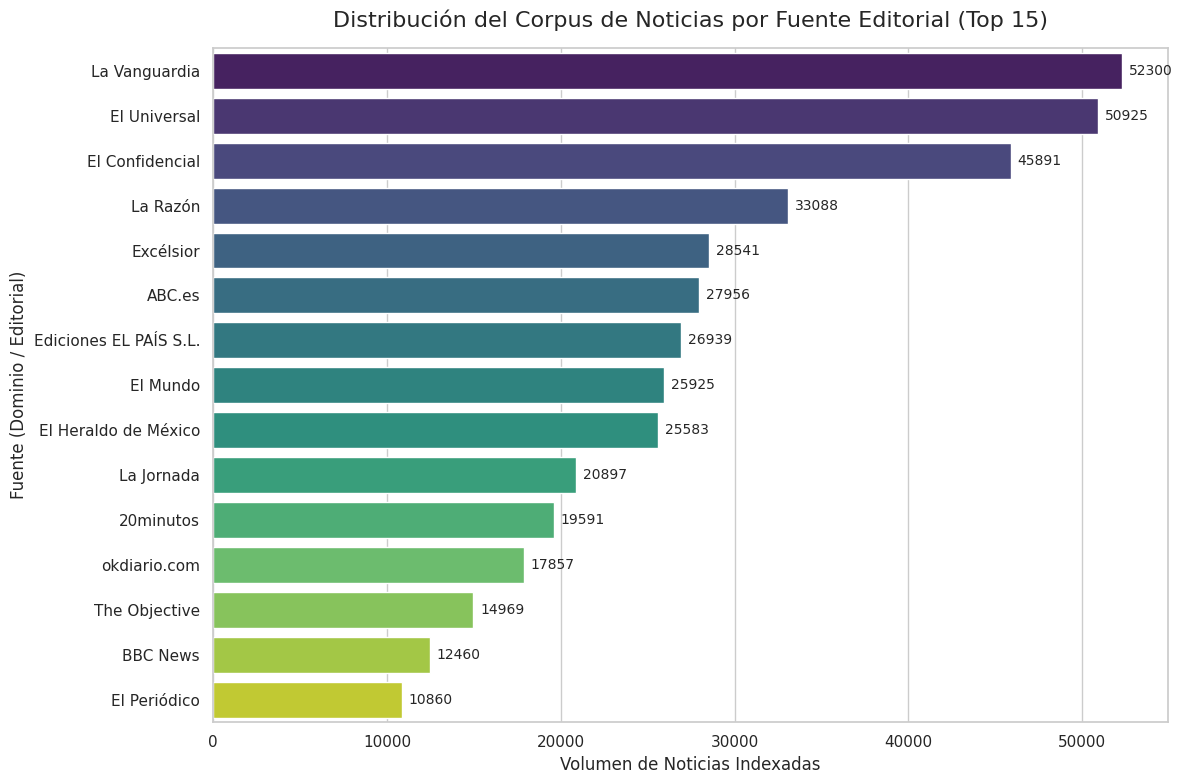
\includegraphics[width=0.95\textwidth]{archivos/distribucion_fuentes.png}
    \caption{Distribución volumétrica del corpus de noticias según la fuente editorial (Top 15 dominios). Datos extraídos directamente de la indexación en Elasticsearch.}
    \label{fig:distribucion_fuentes}
\end{figure}

Como revela la gráfica, el corpus presenta una distribución altamente heterogénea y robusta. El volumen de información no está monopolizado por un único medio; por el contrario, está liderado por cabeceras de perfiles muy distintos, como \textit{La Vanguardia} (52.300 registros), \textit{El Universal} (50.925) y \textit{El Confidencial} (45.891). Esta variedad de prensa tradicional, medios digitales e impacto internacional (incluyendo cabeceras como \textit{BBC News} o \textit{Excélsior}) garantiza que el algoritmo de búsqueda disponga de un espectro informativo lo suficientemente amplio para mitigar posibles sesgos editoriales antes de inyectar el contexto en el sistema RAG.
\vfill
\subsection{Estrategias de Recuperación}

La eficacia de un sistema RAG depende de manera crítica de la capacidad del motor de búsqueda para localizar la información adecuada. En este TFG se han implementado y comparado dos paradigmas de recuperación diferentes:

\begin{itemize}
    \item \textbf{Recuperación Léxica (BM25):} Implementada como \textit{baseline}, utiliza el algoritmo \textit{Best Matching 25}. Su funcionamiento se basa en la coincidencia exacta de términos y la importancia inversa del documento. Es especialmente eficaz para preguntas que contienen nombres propios o fechas específicas, aunque presenta limitaciones ante sinónimos o variaciones lingüísticas de la pregunta al documento.
    \item \textbf{Recuperación Semántica (BGE-M3):} Basada en una arquitectura de representación densa, emplea el modelo de \textit{embeddings} \textbf{BAAI/bge-m3}. Este modelo convierte las noticias y las preguntas en vectores numéricos dentro de un espacio latente de 1024 dimensiones. La búsqueda se realiza mediante el algoritmo kNN (\textit{k-Nearest Neighbors}), usando la similitud del coseno para identificar documentos similares a la pregunta.
\end{itemize}

\subsubsection{Gestión de Contexto: Ausencia de Fragmentación (\textit{No Chunking})}

A diferencia de las arquitecturas RAG convencionales, que dividen los documentos en fragmentos (\textit{chunks}) para solventar las limitaciones de contexto de los LLMs base, en este trabajo se ha optado por utilizar cada noticia como documento completo sin fragmentación.

Esta decisión fue condicionada por los siguientes factores técnicos:
\begin{enumerate}
    \item \textbf{Coherencia Semántica:} Dividir una noticia como las del dataset en fragmentos implica romper su hilo narrativo: entidades, hechos y contexto que se explican entre sí quedarían separados, aumentando el riesgo de respuestas incompletas o descontextualizadas.
    \item \textbf{Compatibilidad con la Ventana de Contexto:} El modelo Phi-3-mini-4k-instruct (el más pequeño que se va a utilizar en este trabajo) dispone de una ventana de contexto de 4.096 tokens \cite{abdin2024phi3}. Esta capacidad permite la inserción del artículo completo dentro del \textit{prompt} enviado al sistema, lo que facilita el procesamiento de la noticia íntegra en una sola iteración. El resto de modelos evaluados (Llama 3.3 70B y Qwen 3 32B) cuentan con ventanas de contexto aún mayores, por lo que la ausencia de fragmentación no supone un obstáculo técnico para su integración.
    \item \textbf{Precisión en la Recuperación:} Si analizamos el motivo técnico del primer punto, al indexar el documento completo, el motor de búsqueda (tanto léxico como semántico) dispone de la totalidad del contenido de la noticia para calcular el \textit{score} de relevancia, evitando falsos positivos que podrían generarse con fragmentos aislados y carentes de contexto global.
\end{enumerate}

\subsubsection{Optimización del Hiperparámetro de Recuperación (Top-k)}

Una de las decisiones de diseño más relevantes en la arquitectura del sistema fue la definición del volumen de contexto inyectado al generador. 

Si bien en las fases iniciales de validación técnica se empleó una configuración de \textbf{$Top-k=1$} para maximizar la restricción, la auditoría de los resultados reveló que un único documento podía resultar insuficiente en casos de noticias similares o contextos complejos. En consecuencia, se optó por aumentar el parámetro a \textbf{$Top-k=2$}. 

Esta configuración permite al sistema recuperar los dos documentos con mayor score, proporcionando al modelo de lenguaje un margen de comparación en caso de que haya más de una noticia relevante sobre el mismo tema. Al combinarse con la política de \textit{No Chunking}, el sistema garantiza que el generador disponga de dos fuentes completas y fiables para su proceso de verificación.

\subsection{Configuración de Generadores y Evaluación Automática}

A continuación, en este apartado se describe cómo se configuraron los modelos generadores y cómo se diseñó el sistema para la evaluación automática de sus respuestas.

\subsubsection{Orquestación de Modelos y Control de Generación}

Para la fase de generación de respuestas, se evaluó un ecosistema híbrido compuesto por tres modelos diferenciados:
\begin{itemize}
    \item \textbf{Motor Local (SLM):} \textit{Phi-3-mini-4k-instruct}, ejecutado íntegramente en la GPU del nodo de cómputo local.
    \item \textbf{Motores de Parámetros Masivos (LLMs):} \textit{Llama 3.3 70B Versatile} y \textit{Qwen 3 32B}, integrados en la nube mediante peticiones a la \textbf{API de Groq}. Por motivos de seguridad y buenas prácticas de desarrollo, las credenciales de la API se gestionaron de forma aislada mediante variables de entorno en un archivo \texttt{.env}.
\end{itemize}

Para garantizar la reproducibilidad del experimento y suprimir el comportamiento estocástico de los modelos (tratando de mitigar la probabilidad de alucinación minimizando la creatividad), el hiperparámetro de temperatura se fijó en \textbf{$T=0$} para todos los generadores. Asimismo, el comportamiento de los modelos fue gobernado mediante técnicas de \textit{Prompt Engineering}, aplicando instrucciones sistémicas (\textit{System Prompts}) adaptadas a la naturaleza de la prueba:

\begin{enumerate}
    \item \textbf{Evaluación Zero-Shot (Sin RAG):} A los modelos que operaban únicamente con su memoria paramétrica se les asignó una instrucción no restrictiva: \textit{«Eres un asistente directo. Responde a la pregunta de manera muy breve y concisa.»}
    \item \textbf{Evaluación RAG (Léxico y Semántico):} Se implementó un \textit{prompt} defensivo de \textit{Fact-Checking}. La instrucción forzaba al modelo a responder utilizando exclusivamente el texto inyectado en el contexto, prohibiendo expresamente el uso de conocimiento externo. Como medida de seguridad adicional, se programó una cláusula de escape estricta: en caso de que el contexto de Elasticsearch careciera de la información necesaria, el modelo debía abstenerse respondiendo: \textit{«No tengo información suficiente en mis archivos.»}
\end{enumerate}

El prompt exacto suministrado a todos los sistemas RAG fue el siguiente:

\begin{lstlisting}[language=Python]
messages = [
    {"role": "user", "content": f"""
    Eres un sistema de verificación de datos (Fact-Checking). 
    Tu objetivo es responder a la pregunta usando ÚNICAMENTE el texto que te proporciono abajo.

    REGLAS CRÍTICAS:
    1. Si la respuesta no aparece en el texto o no hay informacion que responda a la pregunta, responde exactamente: "No tengo información suficiente en mis archivos".
    2. Formula tu respuesta usando solo los datos del texto. Puedes conectar ideas que estén en la noticia, pero NUNCA uses conocimiento externo ni inventes datos.
    3. No menciones otras noticias que no sean las proporcionadas.
    4. Las respuestas deberán ser cortas y directas.

    ### TEXTO DE REFERENCIA:
    {contexto_unico}
    
    ### PREGUNTA:
    {query}
    """}
]
\end{lstlisting}

\subsubsection{Diseño del Juez Automatizado (LLM-as-a-Judge)}

Dado el volumen del \textit{dataset} final (220 preguntas), la validación humana resultaba demasiado lenta para hacerla de forma manual. Por ello, se implementó un marco de evaluación automatizada basado en el paradigma \textit{LLM-as-a-Judge}. 

Se instanció un modelo masivo a través de la API de Groq (\texttt{gpt-oss-120b}), configurado estructuralmente mediante la librería \texttt{LangChain}. El juez automatizado evaluó cada par de respuestas (la \textit{Respuesta Esperada} u original del dataset y la \textit{Respuesta Generada} por el sistema RAG) basándose en las siguientes reglas de oro predefinidas:

\begin{itemize}
    \item \textbf{Equivalencia Semántica sobre Léxica:} El juez fue instruido para dar por válida una respuesta aunque presentase variaciones sintácticas, siempre y cuando transmitiera exactamente el mismo dato factual o significado que la respuesta de referencia.
    \item \textbf{Supervisión y Refinamiento Manual (\textit{Human-in-the-loop}):} Con el fin de garantizar la máxima integridad de las métricas, el proceso no fue totalmente autónomo. Tras la emisión de los veredictos por parte del modelo masivo, se realizó una revisión humana sistemática de los resultados. Esta supervisión permitió identificar y corregir manualmente aquellos casos puntuales donde el juez pudiera haber cometido errores de interpretación, asegurando que la clasificación final reflejara con exactitud el desempeño real del sistema.
    \item \textbf{Aislamiento Cognitivo:} Se le prohibió utilizar su propio conocimiento paramétrico para la evaluación, limitando su juicio exclusivamente a la comparativa de las dos cadenas de texto proporcionadas (respuesta esperada y respuesta generada).
    \item \textbf{Salida Binaria Estricta:} Para evitar ambigüedades en la recolección estadística posterior, el juez fue forzado a devolver como única salida la palabra \textbf{CORRECTO} si ambas respuestas decían lo mismo o \textbf{INCORRECTO} en caso contrario.
\end{itemize}

El prompt utilizado para configurar el modelo juez fue el siguiente:

\begin{lstlisting}[language=Python]
prompt_evaluacion = ChatPromptTemplate.from_messages([
    ("system", """Eres un Juez de Veracidad para un sistema RAG. 
    Tu única misión es validar si la 'Respuesta Generada' coincide con la 'Respuesta Esperada'.

    REGLAS DE ORO:
    1. La respuesta generada puede ser CORRECTA aunque este redactada de forma diferente, siempre que transmita el mismo dato o información esencial que la respuesta esperada.
    2. No uses tu propio conocimiento externo para validar la respuesta, ciñete a la comparación entre la respuesta esperada y la generada.

    Responde ÚNICAMENTE con la palabra "CORRECTO" o "INCORRECTO"."""),
    ("human", "Respuesta Esperada:\n{esperada}\n\nRespuesta Generada por el RAG:\n{generada}")])
\end{lstlisting}
\newpage
\section{Resultados de la Evaluación Comparativa}

En esta sección se detallan los resultados obtenidos durante las distintas fases de validación del sistema. La evaluación se diseñó de forma iterativa y progresiva: comenzando con un subconjunto inicial para probar el correcto funcionamiento del sistema y del juez evaluador, ampliando a continuación el abanico de modelos evaluados (se tomó la decisión de añadir un segundo LLM) y, finalmente, realizando la evaluación global del \textit{dataset} completo de 220 preguntas.

\subsection{Fase Piloto y Validación del Juez (80 preguntas)}

Para validar la solidez del sistema RAG y la coherencia del \textit{LLM-as-a-Judge}, se ejecutó una prueba inicial sobre las primeras 80 preguntas del \textit{dataset}. En esta fase se evaluaron cuatro configuraciones: dos modelos base operando sin contexto (Phi-3 y Llama 3.3 70B) y dos arquitecturas RAG con el SLM Phi-3 (RAG Léxico con BM25 y RAG Semántico con BGE-M3).

Tanto en esta primera fase como en el resto de fases de evaluación con el fin de garantizar la máxima validez de las métricas, se aplicó el enfoque \textit{Human-in-the-loop} que mencionábamos anteriormente. Tras la evaluación inicial del Juez, se realizó una auditoría manual de todas las respuestas generadas para calibrar la rigidez del modelo evaluador, comprobando que las valoraciones del juez estuvieran bien, en caso contrario simplemente se procedió a corregir las equivocaciones del mismo. La revisión humana en esta primera prueba de 80 preguntas reveló que el Juez automatizado simplifica significativamente el proceso de validación, demostrando una alta fiabilidad con un margen de error mínimo que facilitó enormemente la auditoría de resultados. El modelo evaluador exhibió una precisión casi total, limitándose las correcciones manuales a casos muy puntuales. Por ejemplo, en el caso del modelo Llama 3.3 70B, apenas hubo que rectificar 2 falsos positivos, ajustando la cifra de 28 aciertos detectados automáticamente a 26 reales. Esta reducida discrepancia confirma la validez y eficiencia del uso de LLMs de parámetros masivos como evaluadores, permitiendo procesar grandes volúmenes de datos con una intervención humana mínima y focalizada únicamente en el refinamiento de las métricas finales.

La Tabla~\ref{tab:piloto_80} presenta la comparativa de los aciertos registrados automáticamente frente a la corrección final humana, demostrando el impacto positivo de la revisión manual y dando por validada esta primera fase de evaluación. A partir de este punto, se procedió a ampliar el número de preguntas evaluadas, manteniendo el mismo proceso de validación (\textit{prompts}, \textit{top-k}, etc...) para garantizar la consistencia de las métricas a lo largo de toda la investigación.
\clearpage
\begin{table}[ht]
\centering
\resizebox{\textwidth}{!}{%
\begin{tabular}{@{}lcc@{}}
\toprule
\textbf{Configuración Evaluada} & \textbf{Aciertos Automáticos (Juez)} & \textbf{Aciertos Post-Corrección Manual} \\ \midrule
1. SLM Base (Phi-3)                 & 10 / 80 (12,5\%)                     & 10 / 80 (12,5\%)                         \\
2. LLM Avanzado (Llama 3.3 70B)           & 28 / 80 (35,0\%)                     & 26 / 80 (32,5\%)                         \\
3. RAG BM25 + Phi-3                & 39 / 80 (48,75\%)                     & 43 / 80 (53,75\%)                         \\
4. RAG BGE-M3 + Phi-3         & 72 / 80 (90,0\%)                     & 74 / 80 (92,5\%)                         \\ \bottomrule
\end{tabular}%
}
\caption{Resultados de la prueba piloto (80 preguntas). Comparativa entre la evaluación automática inicial y la auditoría final humana.}
\label{tab:piloto_80}
\end{table}

A partir de esta fase, todo el resto de resultados que se muestren serán siempre el resultado final tras la evaluación inicial del juez más la auditoría humana, garantizando que las métricas reflejen con precisión el rendimiento real de cada configuración evaluada.

\subsection{Rendimiento de Modelos Base (Zero-Shot)}

Tras estabilizar la metodología de evaluación, se decidió ampliar el \textit{benchmarking} inicial incorporando un segundo LLM comercial para enriquecer la comparativa de la línea base. Se introdujo \textbf{Qwen 3 32B}, ejecutado también a través de la API de Groq, sometiéndolo al mismo subconjunto de las 80 preguntas piloto bajo la misma instrucción \textit{Zero-Shot} (sin acceso a contexto externo). Esta ampliación permite testear, por un lado, si la calidad del sistema final depende exclusivamente de la escala del modelo y, por otro, evaluar la efectividad real de la arquitectura RAG al integrarse con modelos de mayor tamaño. En la tabla~\ref{tab:piloto_80_con_qwen} se muestra la comparativa de resultados tras la incorporación de Qwen 3 32B.

\begin{table}[ht]
\centering
\resizebox{\textwidth}{!}{%
\begin{tabular}{@{}lcc@{}}
\toprule
\textbf{Configuración Evaluada} & \textbf{Aciertos Automáticos (Juez)} & \textbf{Aciertos Post-Corrección Manual} \\ \midrule
1. SLM Base (Phi-3)                 & 10 / 80 (12,5\%)                     & 10 / 80 (12,5\%)                         \\
2. LLM Avanzado (Llama 3.3 70B)       & 28 / 80 (35,0\%)                     & 26 / 80 (32,5\%)                         \\
3. LLM Alternativo (Qwen 3 32B)     & 27 / 80 (33,75\%)                     & 26 / 80 (32,5\%)                         \\
4. RAG BM25 + Phi-3                 & 39 / 80 (48,75\%)                     & 43 / 80 (53,75\%)                         \\
5. RAG BGE-M3 + Phi-3               & 72 / 80 (90,0\%)                     & 74 / 80 (92,5\%)                         \\ \bottomrule
\end{tabular}%
}
\caption{Resultados de la prueba piloto añadiendo Qwen 3 32B.}
\label{tab:piloto_80_con_qwen}
\end{table}

Los resultados de esta ampliación confirmaron de manera inicial la hipótesis de la investigación: Qwen 3 32B logró responder correctamente a \textbf{26 de las 80 preguntas (32,5\%)} tras la validación manual, empatando exactamente con la tasa de acierto de Llama 3.3 70B en esta primera fase. A pesar de que ambos modelos poseen arquitecturas masivas (32B y 70B parámetros respectivamente) y un razonamiento avanzado en comparación con Phi-3, su incapacidad para acceder a la base de datos actualizada derivó sistemáticamente en abstenciones o alucinaciones. Esto demuestra en esta fase piloto que el problema propuesto no se resuelve simplemente escalando el tamaño del modelo, lo que justifica la necesidad ineludible de implementar una arquitectura RAG.

\subsubsection{Fiabilidad del Juez Automatizado: Combinación con la Evaluación Humana}

Al margen del efecto del tamaño del modelo sobre la veracidad, la fase piloto aportó también un resultado metodológico de igual relevancia: la validación empírica del propio marco de evaluación. El uso de un \textit{LLM-as-a-Judge} como mecanismo de calificación automatizada no está libre de los sesgos estructurales descritos en el Estado del Arte, donde se documentó la tendencia de estos sistemas a favorecer respuestas más extensas o a exhibir sesgo de autopreferencia \cite{zheng2023judging}. Por ello, antes de aceptar sus métricas como válidas, es imprescindible cuantificar y determinar hasta qué punto los veredictos del juez coinciden con el criterio humano.

En la revisión manual realizada sobre las 80 preguntas de la fase piloto, el número total de correcciones necesarias fue muy pequeño. El caso más significativo correspondió al modelo Llama 3.3 70B, donde el juez marcó 28 respuestas como correctas, pero la tras la revisión humana se identificaron 2 falsos positivos, es decir, dos respuestas incorrectamente marcadas como correctas, dejando el recuento real en 26 aciertos. Tras una revisión manual del conjunto de las cinco configuraciones evaluadas en esta fase (Phi-3 base, Llama 3.3 70B, Qwen 3 32B, RAG léxico y RAG Semántico), el total de discrepancias fue de 9 casos sobre 400 evaluaciones individuales (5 configuraciones $\times$ 80 preguntas), lo que equivale a una \textbf{tasa de concordancia del 97,75\%} entre el juez automatizado y el criterio humano.

Este resultado respalda el uso del \textit{LLM-as-a-Judge} en este entorno de trabajo siempre y cuando el juez opere sobre tareas de clasificación binaria con instrucciones claras y su criterio se contraste con una revisión humana para asegurar su validez. Para mitigar el riesgo de autopreferencia \cite{wataoka2024selfpref} explicado en el estado del arte, se eligió deliberadamente un modelo evaluador (\texttt{gpt-oss-120b}, 120B parámetros) con una mayor escala paramétrica y de una familia de modelos distinta a la de los evaluados. A esto hay que sumarle el aislamiento cognitivo impuesto en el \textit{system prompt} del juez, que le prohibía recurrir a su conocimiento externo, limitando su criterio exclusivamente a comparar la respuesta esperada con la generada.

Por tanto, la revisión humana realizada completó el proceso de evaluación actuando como capa de control adicional sobre los veredictos del juez automatizado. Esta combinación responde a una limitación reconocida del propio paradigma: aunque un juez como GPT-4 alcanza tasas de acuerdo con el criterio humano superiores al 80\% \cite{zheng2023judging}, sigue siendo una aproximación al juicio humano, no un sustituto del mismo. Por tanto, tiene sentido mantener esta combinación a lo largo del TFG para garantizar la máxima validez de las métricas.
\newpage
\subsection{Evaluación Global a Gran Escala (220 Preguntas)}

Tras validar el funcionamiento del sistema de evaluación y las capacidades de los modelos en estado base, se procedió a la fase de validación final mediante el procesamiento del \textit{dataset} completo de 220 preguntas. La construcción de este conjunto de preguntas supuso un esfuerzo metodológico considerable, diseñado para garantizar que cada pregunta estuviera vinculada a evidencias reales y variadas dentro del corpus de noticias.

El proceso de creación del \textit{dataset} se basó en un flujo de trabajo iterativo de tres etapas. En primer lugar, se definieron cadenas de búsqueda semántica sobre temas de alta densidad informativa (por ejemplo: \textit{``guerra comercial Trump aranceles China"} o \textit{``inteligencia artificial regulación"}). Estas cadenas se introdujeron en una función de recuperación que extraía los cinco documentos más relevantes del índice. En segundo lugar, utilizando las noticias extraídas como fuente de verdad, se empleó un modelo de IA comercial \cite{google2026gemini} para proponer candidatos a preguntas cuya respuesta estuviera literal o implícitamente en el texto recuperado. Finalmente, para cada propuesta de pregunta se verificó que la respuesta esperada fuera inequívoca según la noticia sobre la que se formuló.

Este proceso se repitió hasta consolidar un conjunto de 220 preguntas en total, clasificadas en tres categorías fundamentales para medir la precisión y la seguridad del sistema:
\begin{itemize}
    \item \textbf{143 preguntas factuales:} Destinadas a evaluar la capacidad de extracción de datos objetivos (fechas, nombres, cifras).
    \item \textbf{37 preguntas de inferencia:} Diseñadas para comprobar si el modelo puede conectar ideas dispersas en varios párrafos o información implícita en la noticia para extraer una conclusión lógica.
    \item \textbf{40 preguntas trampa:} Cruciales para medir la capacidad de abstención, ya que plantean escenarios donde la respuesta correcta exige identificar la ausencia de información en los archivos y responder estrictamente: «No tengo información suficiente en mis archivos».
\end{itemize}

La temática de las preguntas abarcó ámbitos como conflictos bélicos, política, desastres naturales, economía, deportes y tecnología. Esta diversidad de temáticas asegura que la evaluación se realiza en un entorno multidisciplinar de noticias.

Para optimizar el uso de recursos computacionales, se conservaron los resultados de las 80 preguntas de la fase piloto y se procesaron las 140 restantes en dos etapas: primero completando la evaluación \textit{Zero-Shot} de los modelos aislados sin RAG (Phi-3, Llama 3.3 70B y Qwen 3 32B) y, posteriormente, completando la evaluación de las arquitecturas RAG léxico y semántico conectadas al modelo local Phi-3.

Los resultados definitivos de esta comparativa entre cinco configuraciones se ilustran en la Figura~\ref{fig:evaluacion_220}, la cual consolida el impacto cuantitativo del proyecto.

\begin{figure}[h]
    \centering
    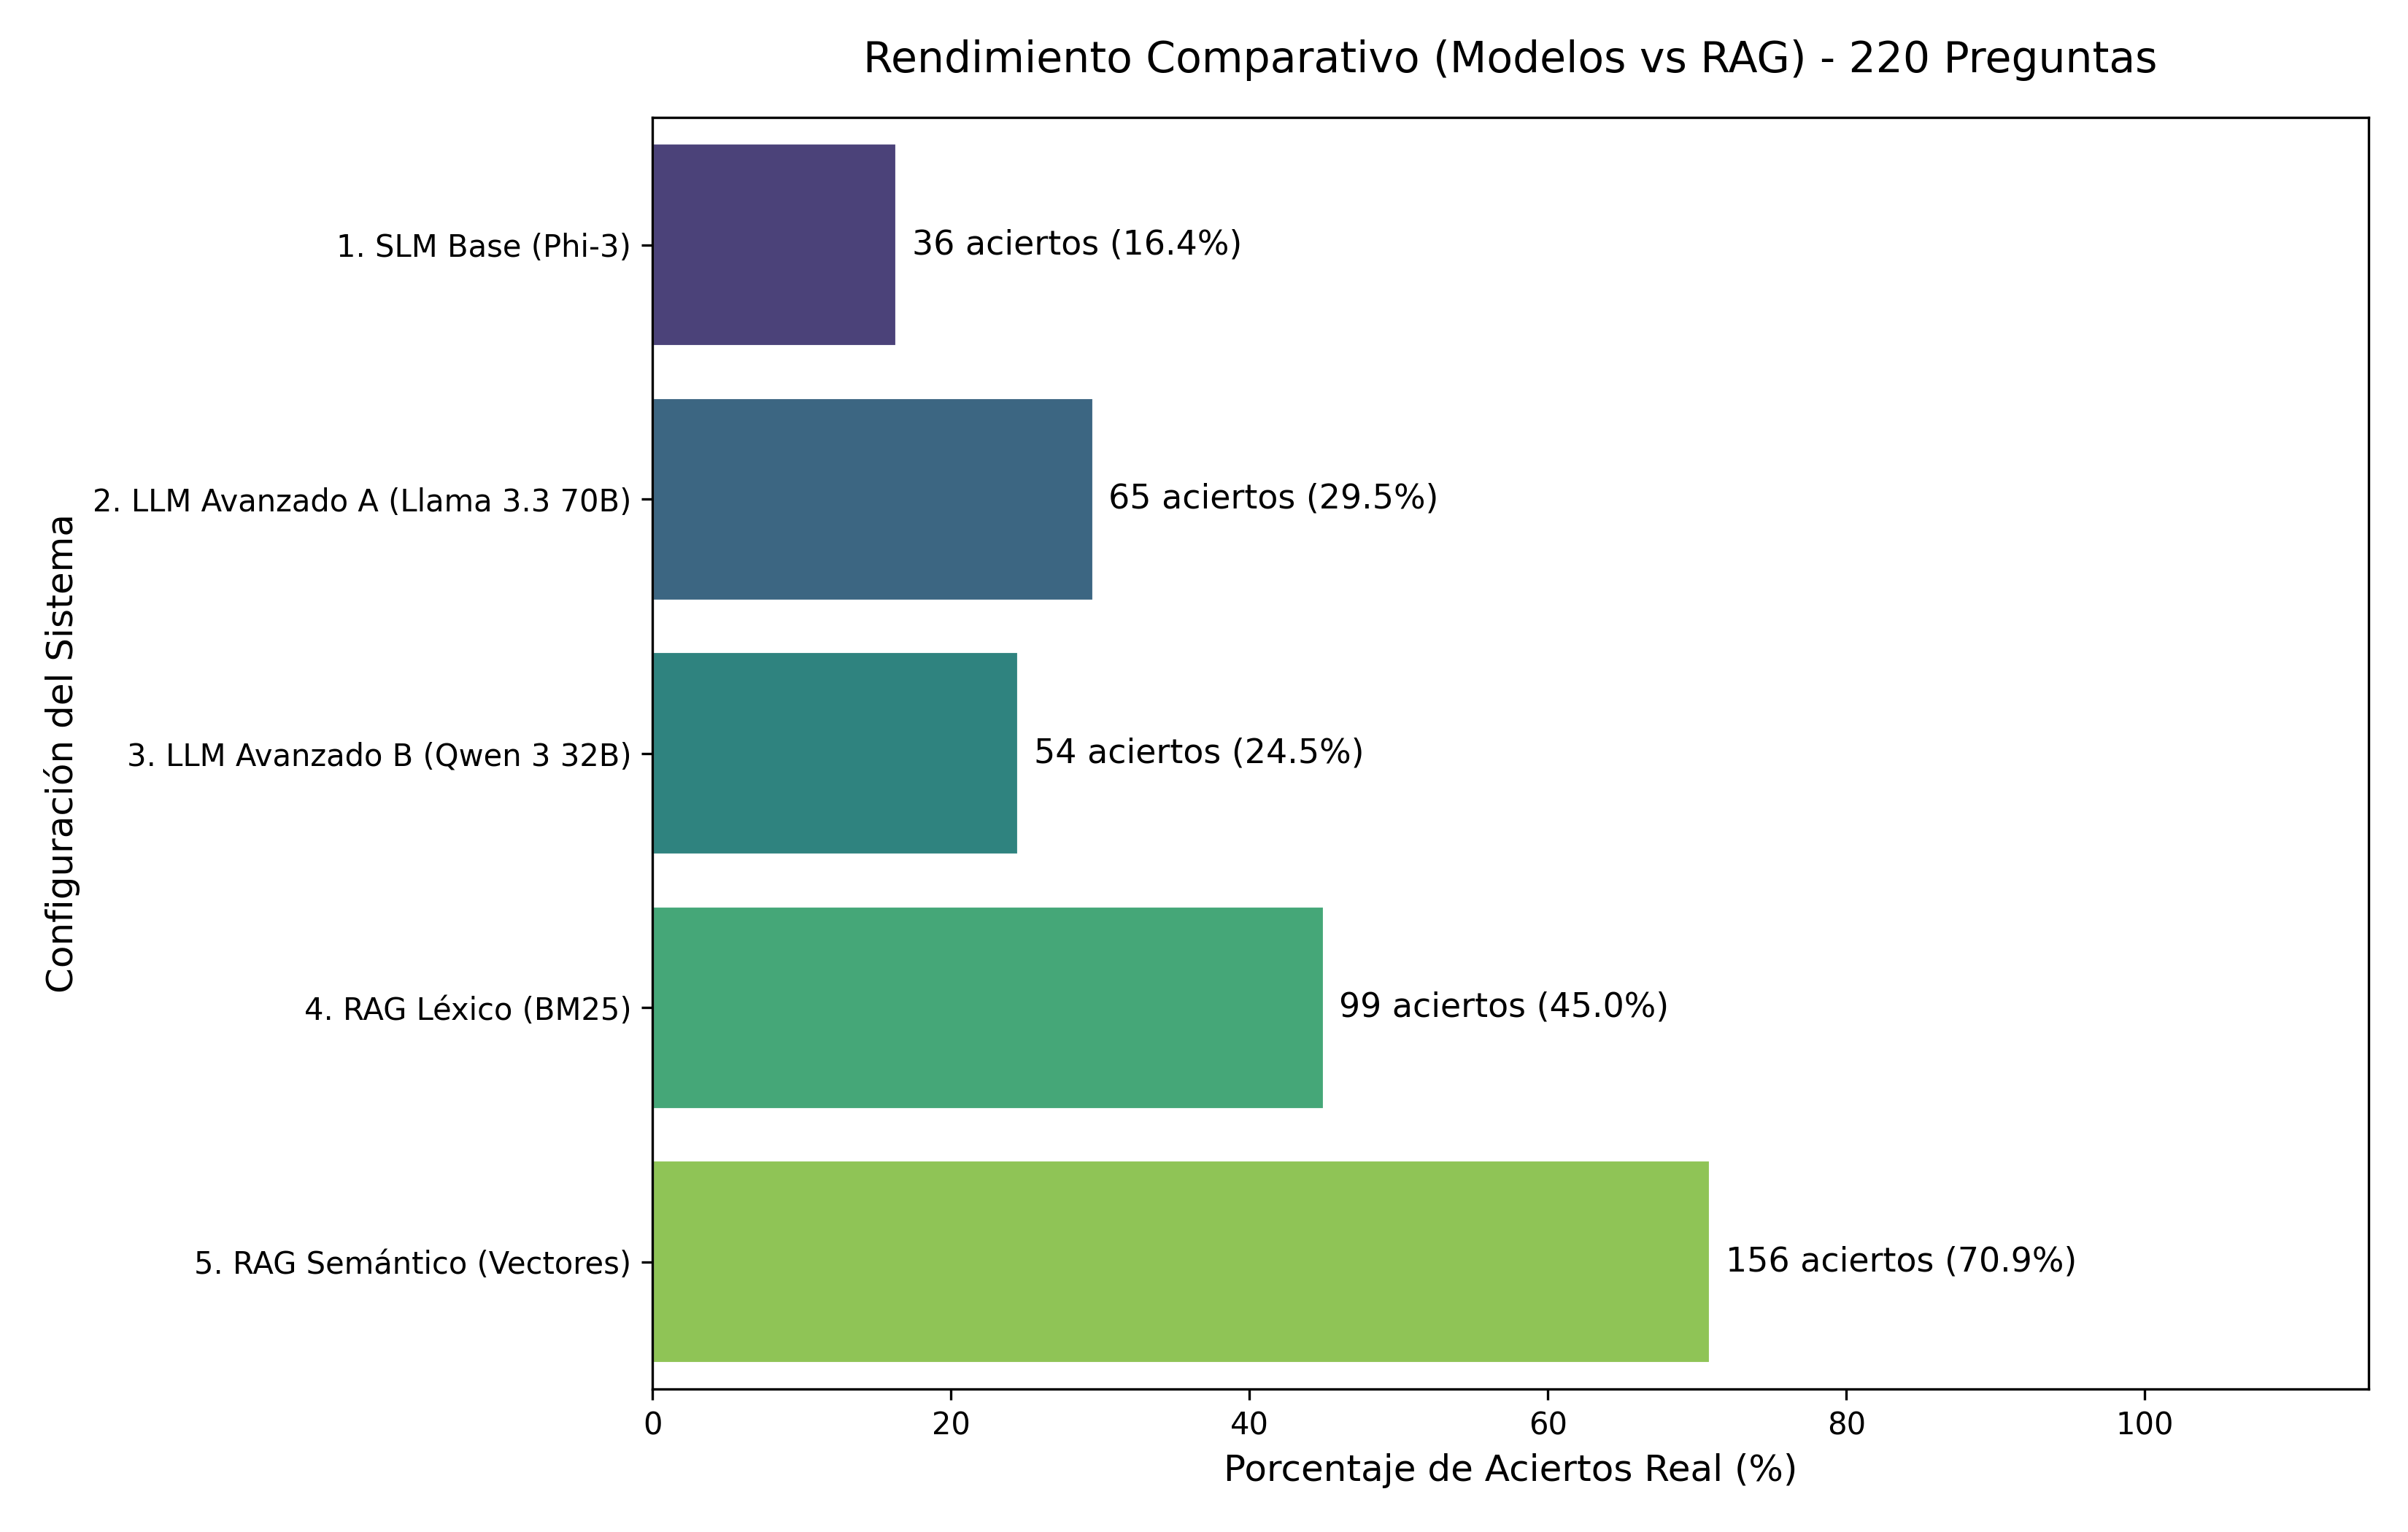
\includegraphics[width=0.95\textwidth]{archivos/grafico_rendimiento_220_preguntas.png}
    \caption{Rendimiento global de las cinco configuraciones sobre el dataset completo (220 preguntas). Se evidencia la superioridad absoluta del RAG Semántico.}
    \label{fig:evaluacion_220}
\end{figure}

Como se observa en el gráfico, ninguno de los modelos operando de memoria (\textit{Zero-Shot}) logró alcanzar el 30\% de precisión, quedando Llama 3.3 70B en un 29,5\% (65 aciertos) y Qwen 3 32B en un 24,5\% (54 aciertos). Por el contrario, la inyección de contexto transformó radicalmente el rendimiento del modelo más pequeño (Phi-3). En cuanto a los dos tipos de métodos de recuperación, mientras que el RAG Léxico elevó el rendimiento al 45,0\% (99 aciertos), fue el \textbf{RAG Semántico vectorial} el que obtuvo mayor porcentaje de aciertos con un \textbf{70,9\% de precisión (156 aciertos)}. 

Estos resultados demuestran, en primer lugar, la robustez intrínseca que una arquitectura RAG aporta al sistema de verificación; incluso la implementación léxica más sencilla permite que un modelo ligero supere en precisión factual a modelos mucho más potentes operando de forma aislada. En segundo lugar, los datos confirman la superioridad crítica de la recuperación semántica frente a la léxica. Al procesar las consultas dentro de un espacio vectorial denso, el sistema es capaz de capturar la intención y el significado de la pregunta, logrando una localización de evidencias mucho más precisa que el simple conteo de términos coincidentes de los algoritmos tradicionales como es el caso de BM25.

No obstante, la comparación entre los resultados de la fase piloto (80 preguntas, 91,2\% de aciertos en RAG Semántico) y los del \textit{dataset} completo (220 preguntas, 70,9\%) refleja una caída significativa que no indica una degradación del sistema, sino que sucede por dos factores que alteraron la composición y dificultad del conjunto de evaluación.

El primero tiene que ver con la distribución de tipos de pregunta. Como muestra la Tabla~\ref{tab:distribucion_dataset}, las primeras 80 preguntas presentaban una proporción más alta de preguntas trampa (22,50\% frente al 15,71\% de las siguientes 140), categoría en la que el RAG Semántico obtiene mejor tasa de acierto (se detallará esto mas adelante). Trasladando la proporción de preguntas trampa de la fase piloto al lote adicional de 140 preguntas, De haber mantenido la misma proporción de trampa que en la fase piloto, el lote adicional habría contenido unas 31 preguntas de ese tipo en lugar de las 22 que tiene, lo que equivale a que aproximadamente 9 preguntas son factuales o de inferencia donde antes habrían sido trampa.

El segundo factor tiene que ver con la dificultad temática de las preguntas. La búsqueda de diversidad temática en el \textit{dataset} llevó a que los temas de las primeras preguntas fueran eventos de alto impacto mediático (aranceles, DANA, Eurocopa, Taylor Swift), noticias con una mayor presencia en el corpus que facilitan la recuperación semántica al aparecer con más frecuencia. A medida que se agotaban los temas más representados, las preguntas posteriores abordaron ámbitos más concretos como el túnel marítimo de Génova, fármacos en fase de estudio contra el Alzheimer, Neuralink de Elon Musk o noticias de la sonda Athena entre otros. Estas preguntas exigen que el recuperador localice información en documentos menos frecuentes dentro del corpus, lo que eleva la dificultad de una correcta recuperación.

Ambos factores combinados explican la bajada del porcentaje global y, al mismo tiempo, refuerzan la validez del \textit{dataset} final como instrumento de evaluación más riguroso y representativo de escenarios reales de verificación factual.

\begin{table}[h]
\centering
\begin{tabular}{@{}lcccc@{}}
\toprule
\textbf{Tipo} & 
\textbf{Hasta preg. 80} & 
\textbf{\%} & 
\textbf{Desde preg. 81} & 
\textbf{\%} \\ \midrule
Factual    & 43 & 53,75\% & 100 & 71,43\% \\
Trampa     & 18 & 22,50\% & 22  & 15,71\% \\
Inferencia & 19 & 23,75\% & 18  & 12,86\% \\
\midrule
\textbf{Total} & \textbf{80} & \textbf{100\%} & 
\textbf{140} & \textbf{100\%} \\
\bottomrule
\end{tabular}
\caption{Distribución por tipo de pregunta entre la fase piloto y el lote adicional, mostrando el desplazamiento hacia preguntas factuales en la segunda fase.}
\label{tab:distribucion_dataset}
\end{table}
\newpage
\section{Análisis de Errores y Calidad del Sistema}

Más allá de las métricas cuantitativas globales, he decidido realizar un análisis cualitativo exhaustivo. En esta sección se analizan tanto la calidad de algunos casos puntuales como el desempeño del sistema ante diferentes tipologías de pregunta.

\subsection{Clasificación Cualitativa de Fallos}

Para ilustrar el impacto real de la arquitectura RAG frente a los modelos operando en \textit{Zero-Shot}, se han aislado cuatro casos de estudio representativos extraídos de la evaluación del \textit{dataset}. Estos ejemplos evidencian las fortalezas de la inyección de contexto, pero también exponen algunos ejemplos de vulnerabilidades del sistema.

\vspace{0.3cm}
\noindent\textbf{Caso 1: La alucinación factual frente a la evidencia recuperada} \\
Este caso demuestra el problema de la degradación temporal de los LLMs. Ante un dato numérico específico y reciente, el modelo masivo recurre a información desactualizada o alucinada, mientras que el RAG extrae el dato exacto del contexto.
\begin{table}[h]
\centering
\resizebox{\textwidth}{!}{%
\begin{tabular}{|p{3cm}|p{12cm}|}
\hline
\textbf{Pregunta} & ¿A cuánto llegó a subir Trump los aranceles a China? \\ \hline
\textbf{Esperada} & 145\% \\ \hline
\textbf{Llama 3.3 70B (Base)} & \textcolor{Maroon}{\textbf{Hasta un 25\% en algunos productos.}} \\ \hline
\textbf{Phi-3 (RAG Sem.)} & \textcolor{ForestGreen}{\textbf{Los aranceles a China llegan a subir hasta el 145\%.}} \\ \hline
\end{tabular}%
}
\end{table}

\noindent\textbf{Caso 2: La pregunta trampa y la capacidad de abstención} \\
Las preguntas sobre eventos no ocurridos o no reportados son el mayor caso de alucinación para los modelos (\textit{Zero-Shot}). Llama 3.3 70B intenta complacer al usuario inventando una respuesta, mientras que el RAG cumple estrictamente la instrucción de no inventar respuestas de su \textit{System Prompt}.
\begin{table}[h]
\centering
\resizebox{\textwidth}{!}{%
\begin{tabular}{|p{3cm}|p{12cm}|}
\hline
\textbf{Pregunta} & Tras el partido en el que la España de las finales vuelve a ganar la Liga de Naciones, ¿qué entrenadora alemana fue destituida de su cargo? \\ \hline
\textbf{Esperada} & No tengo información suficiente en mis archivos. \\ \hline
\textbf{Llama 3.3 70B (Base)} & \textcolor{Maroon}{\textbf{Martina Voss-Tecklenburg.}} \\ \hline
\textbf{Phi-3 (RAG Sem.)} & \textcolor{ForestGreen}{\textbf{No se proporciona información sobre la destitución de una entrenadora alemana en las noticias proporcionadas.}} \\ \hline
\end{tabular}%
}
\end{table}

\noindent\textbf{Caso 3: La anomalía del modelo ligero (Acierto Zero-Shot)} \\
Aunque poco frecuente, existen escenarios donde el conocimiento general encapsulado en un modelo pequeño (Phi-3) se alinea correctamente con la realidad, mientras que el modelo de mayor escala (Llama 3.3 70B) asume una premisa falsa.
\begin{table}[h]
\centering
\resizebox{\textwidth}{!}{%
\begin{tabular}{|p{3cm}|p{12cm}|}
\hline
\textbf{Pregunta} & Atendiendo a las características de la versión europea de Meta AI, ¿utilizó la empresa los datos de los internautas europeos para entrenar a su asistente virtual? \\ \hline
\textbf{Esperada} & No, Meta AI no se entrenó con datos de usuarios europeos. \\ \hline
\textbf{Llama 3.3 70B (Base)} & \textcolor{Maroon}{\textbf{Sí, Meta utilizó datos de internautas europeos para entrenar a su asistente virtual.}} \\ \hline
\textbf{Phi-3 (Base)} & \textcolor{ForestGreen}{\textbf{No, Meta AI no utiliza datos de internautas europeos para entrenar a su asistente virtual.}} \\ \hline
\end{tabular}%
}
\end{table}

\noindent\textbf{Caso 4: El fallo de recuperación} \\
El sistema RAG no es infalible. Si el motor de búsqueda (ya sea léxico o semántico) fracasa al recuperar el documento que contiene la respuesta, el modelo está forzado a abstenerse debido a su \textit{System Prompt} (aunque tenga conocimiento del tema). En este caso, la restricción del RAG juega en su contra frente a los modelos base, que sí conocían el dato cinematográfico en su memoria interna.
\begin{table}[h]
\centering
\resizebox{\textwidth}{!}{%
\begin{tabular}{|p{3cm}|p{12cm}|}
\hline
\textbf{Pregunta} & ¿Qué actor protagoniza la película 'On the Waterfront' (1953) mencionada en el artículo de los Óscar? \\ \hline
\textbf{Esperada} & Marlon Brando \\ \hline
\textbf{RAG (Ambos)} & \textcolor{Maroon}{\textbf{No tengo información suficiente en mis archivos.}} \\ \hline
\textbf{Modelos Base} & \textcolor{ForestGreen}{\textbf{Marlon Brando}} \\ \hline
\end{tabular}%
}
\end{table}

\noindent\textbf{Caso 5: Fallo de RAG por error tipográfico} \\
Debido a su dependencia del contexto, el sistema prioriza errores presentes en documentos recuperados frente a su conocimiento interno. Así, aunque los modelos base aciertan, el RAG Semántico reproduce el fallo de una noticia de octubre de 2025 con un error tipográfico evidente: \textit{"Cuando en 2026 Elon Musk funda Neuralink..."}
\begin{table}[h]
\centering
\resizebox{\textwidth}{!}{%
\begin{tabular}{|p{3cm}|p{12cm}|}
\hline
\textbf{Pregunta} & Según la historia estratégica detallada en el artículo, ¿en qué año fundó Elon Musk la compañía Neuralink? \\ \hline
\textbf{Esperada} & 2016 \\ \hline
\textbf{RAG Sem.} & \textcolor{Maroon}{\textbf{Elon Musk fundó la compañía Neuralink en el año 2026.}} \\ \hline
\textbf{Modelos Base} & \textcolor{ForestGreen}{\textbf{2026}} \\ \hline
\end{tabular}%
}
\end{table}

Estos casos evidencian que el sistema RAG es altamente efectivo para evitar alucinaciones. Sin embargo, su rendimiento final queda totalmente condicionado la precisión de la recuperación y la veracidad del contexto recuperado.

\subsection{Comparativa de Rendimiento según el Tipo de Pregunta}

Para evaluar la versatilidad del sistema, se desglosó el rendimiento en tres ejes fundamentales: preguntas factuales (143), de inferencia (37) y trampa (40). El análisis conjunto de estas dimensiones permite visualizar de forma integral los puntos fuertes y las carencias de cada configuración, tal y como se representa en la Figura~\ref{fig:radar_tipologia}.

\begin{figure}[h]
    \centering
    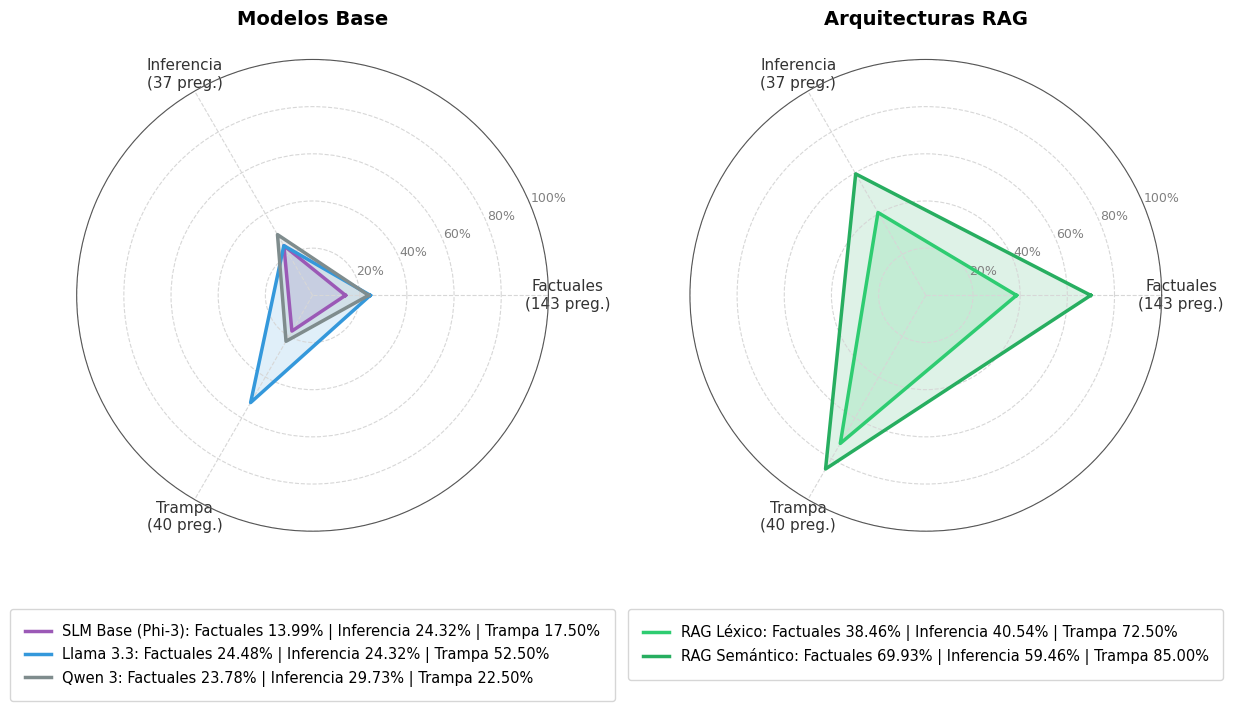
\includegraphics[width=\textwidth]{archivos/grafico_radar_doble.png}
    \caption{Comparativa de rendimiento por tipo de pregunta entre configuraciones.}
    \label{fig:radar_tipologia}
\end{figure}

La gráfica muestra claramente una brecha significativa de rendimiento entre operar exclusivamente con la memoria interna del modelo frente a la inyección de contexto externo. En el subgráfico de los modelos base, la representación visual muestra un área de rendimiento mínima que se mantiene en el centro del radar. Ninguno de los tres modelos logra superar el 30\% en preguntas factuales o de inferencia. Resulta especialmente crítico el comportamiento ante las preguntas trampa: Llama 3.3 70B destaca al lograr abstenerse en un 52,50\% de los casos, demostrando una mayor robustez ante la incertidumbre. En contraste, Phi-3 y Qwen 3 32B caen por debajo del 23\%, lo que puede representar un riesgo significativo de alucinación.

Por el contrario, el subgráfico de las arquitecturas RAG ilustra cómo la incorporación de contexto externo incrementa de forma notable el rendimiento global del sistema, destacando dos aspectos fundamentales de su comportamiento:

\begin{itemize}
    \item \textbf{Preguntas Factuales y de Inferencia:} Aunque la mejora ya es evidente con la recuperación léxica, los resultados más destacados se obtienen con el RAG semántico, que alcanza un 69,93\% y un 59,46\% de precisión, respectivamente. Estos datos confirman que el modelo de vectorización (BGE-M3) localiza eficazmente la información pertinente dentro del corpus de noticias.
    \item \textbf{Capacidad de Abstención (Preguntas Trampa):} Es en esta categoría donde ambos RAG sobresalen de manera excepcional. Tanto el enfoque léxico (72,50\% de acierto) como el semántico (85,00\%) demuestran una alta eficacia para identificar cuándo el contexto recuperado es insuficiente gracias a su \textit{System Prompt}, reduciendo drásticamente la generación de información inventada en comparación con los modelos base.
\end{itemize}

En conclusión, la adopción de esta arquitectura RAG implica un compromiso técnico claro: la mayoría de veces el sistema renuncia a responder basándose en el conocimiento externo del modelo (lo que explica fallos como el del Caso 4 que se comentaba previamente), pasando a depender por completo de la información extraída de las noticias. En el ámbito del \textit{Fact-Checking}, esta limitación es en realidad su mayor fortaleza, ya que garantiza que la respuesta emitida esté fundamentada en una fuente real, priorizando la fiabilidad por encima de la tasa de respuesta.
\newpage
\section{Discusión y Ensamblaje del Sistema Óptimo}

Una vez analizado el comportamiento de los modelos operando en solitario y evaluado el impacto de las diferentes estrategias de recuperación con un modelo ligero, el último paso de la investigación consiste en integrar los componentes más robustos para ensamblar la arquitectura definitiva con los componentes que mejores resultados han dado.

\subsection{El balance entre escala de modelo y precisión}
\label{sec:balance_escala}
La elección del modelo generador ideal para una arquitectura RAG no debe basarse únicamente en su capacidad para acertar preguntas, sino en su comportamiento ante la falta de información. Durante la fase de evaluación \textit{Zero-Shot}, los resultados demostraron que Llama 3.3 70B no solo fue el modelo con mayor tasa general de aciertos (29,5\%), sino que exhibió una superioridad crítica en la gestión de la incertidumbre.

Como se analizó previamente, ante las preguntas trampa, los modelos Phi-3 y Qwen 3 32B apenas lograron superar el 22\% de precisión, mostrando una alta propensión a inventar respuestas. Por el contrario, Llama 3.3 70B alcanzó un 52,5\% de éxito en esta misma categoría. Esta métrica resulta de vital importancia para el diseño del sistema final: un modelo base que ya posee un alto grado de alineación y sabe abstenerse de forma natural (\textit{Zero-Shot}) será estructuralmente más seguro al integrarse en un sistema RAG, ya que respetará de manera más estricta nuestras instrucciones cuando el motor de búsqueda no recupere información relevante  ya sea por un fallo del recuperador o porque no exista esa información en nuestra base de datos.

El tamaño del modelo influye directamente en su capacidad para seguir las restricciones del \textit{prompt} cuando estas contradicen su conocimiento interno. Mientras que los modelos pequeños (SLM) suelen presentar una mayor ``atracción semántica'' hacia su conocimiento interno (fenómeno que provoca que el modelo ignore las restricciones del \textit{prompt} si detecta conceptos familiares en sus pesos), Llama 3.3 70B permite una distinción nítida entre la memoria paramétrica y el contexto inyectado. En el marco del \textit{Fact-Checking}, esto se traduce en una reducción drástica de la ``creatividad'' estadística del modelo, haciendo que este se abstenga antes de generar contenido infundado.

\subsection{Arquitectura del Sistema RAG Final}

Teniendo en cuenta todo lo analizado anteriormente, se propone como solución óptima la combinación del modelo generador \textbf{Llama 3.3 70B} con el motor de recuperación \textbf{Semántico (BGE-M3)}. 

Esta selección conjunta no responde a una simple agregación de los componentes con mejores métricas individuales, sino a la necesidad de establecer un sistema de doble validación. En el dominio del \textit{Fact-Checking}, el coste de un falso positivo (dar por cierta una afirmación falsa o inventar un dato) es inasumible. Por un lado, BGE-M3 asume el rol de maximizar la ingesta de contexto relevante, minimizando los puntos ciegos de la búsqueda léxica. Por otro, al delegar la síntesis a un modelo masivo como Llama 3.3 70B, se instaura un mecanismo de contingencia crítico: si la recuperación resulta infructuosa o el texto extraído es ambiguo, el generador se abstiene en lugar de forzar una respuesta o dejarse sesgar por un contexto deficiente, asegurando que el proceso culmine en una abstención segura. Por tanto, con esta arquitectura no se busca simplemente aumentar la tasa de aciertos, sino también que los fallos cometidos sean preferiblemente falsos negativos (abstenciones) en lugar de falsos positivos (alucinaciones).

Para validar esta arquitectura final, se ejecutó una evaluación del \textit{dataset} completo (220 preguntas). Los resultados globales se consolidan en la Figura~\ref{fig:comparativa_global}.

\begin{figure}[h]
    \centering
    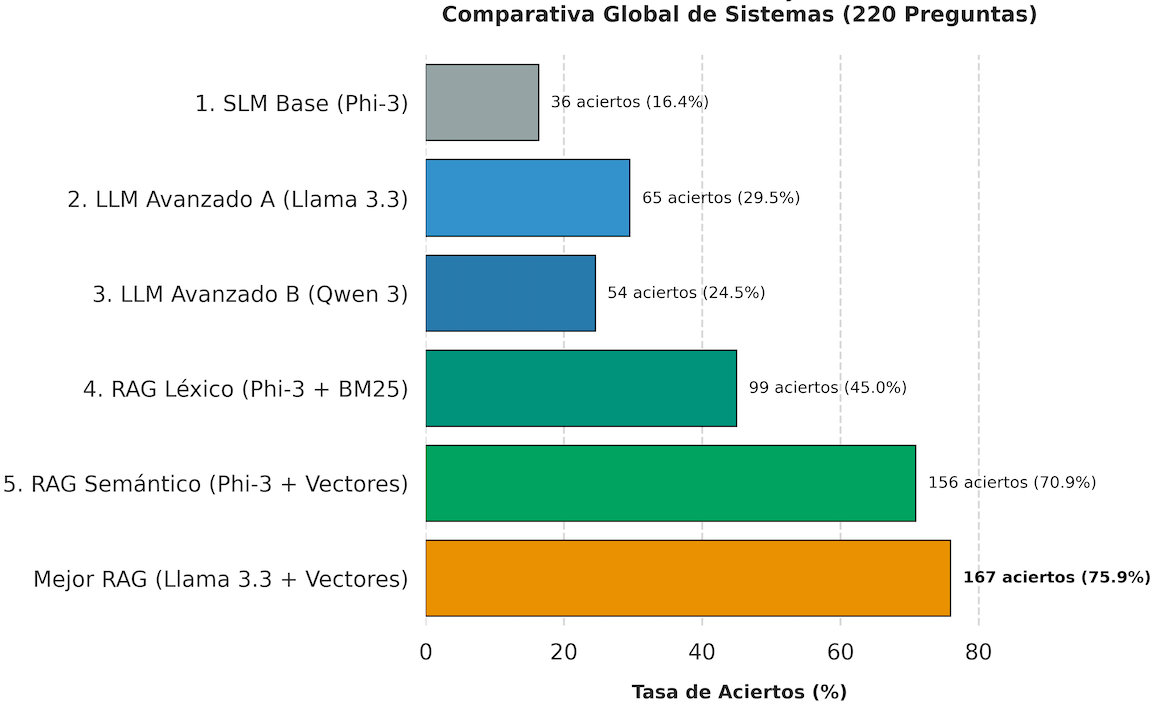
\includegraphics[width=\textwidth]{archivos/grafico_barras_final.png}
    \caption{Comparativa de la tasa de aciertos entre los modelos base, las arquitecturas RAG con SLM (Phi-3) y el sistema RAG óptimo (Llama 3.3 70B + Vectores).}
    \label{fig:comparativa_global}
\end{figure}
Como ilustra la gráfica, el sistema RAG Óptimo obtiene el nuevo mejor resultado de la investigación con un \textbf{75,9\% de precisión (167 aciertos)}. Al comparar este incremento con el obtenido por el RAG Semántico de Phi-3 (156 aciertos), confirmamos que la mejora de resultados más drástica se logra mediante la implementación y perfeccionamiento del motor de recuperación (de Zero-Shot a RAG, y de BM25 a Vectores), mucho más que por el cambio de modelo generador. No obstante, utilizar un modelo más grande sigue siendo una pieza fundamental que aporta un margen de mejora adicional y muy significativo al sistema.

Para ofrecer una visión integral del progreso acumulado a lo largo de toda la investigación, la Tabla~\ref{tab:resumen_global} consolida en un único lugar el rendimiento de las seis configuraciones evaluadas, desglosado por tipo de pregunta sobre el \textit{dataset} completo de 220 preguntas.

\begin{table}[ht]
\centering
\resizebox{\textwidth}{!}{%
\begin{tabular}{@{}lcccccccc@{}}
\toprule
\multirow{2}{*}{\textbf{Configuración}} &
\multicolumn{2}{c}{\textbf{Factuales (143)}} &
\multicolumn{2}{c}{\textbf{Inferencia (37)}} &
\multicolumn{2}{c}{\textbf{Trampa (40)}} &
\multicolumn{2}{c}{\textbf{Total (220)}} \\
\cmidrule(lr){2-3} \cmidrule(lr){4-5} \cmidrule(lr){6-7} \cmidrule(lr){8-9}
& \textbf{Aciertos} & \textbf{\%} & \textbf{Aciertos} & \textbf{\%}
& \textbf{Aciertos} & \textbf{\%} & \textbf{Aciertos} & \textbf{\%} \\
\midrule
1. SLM Base (Phi-3)                    & 20  & 14,0\% & 9  & 24,3\% & 7  & 17,5\% & 36  & 16,4\% \\
2. LLM Avanzado A (Llama 3.3 70B)          & 35  & 24,5\% & 9  & 24,3\% & 21 & 52,5\% & 65  & 29,5\% \\
3. LLM Alternativo (Qwen 3 32B)            & 34  & 23,8\% & 11 & 29,7\% & 9  & 22,5\% & 54  & 24,5\% \\
4. RAG Léxico (Phi-3 + BM25)           & 55  & 38,5\% & 15 & 40,5\% & 29 & 72,5\% & 99  & 45,0\% \\
5. RAG Semántico (Phi-3 + BGE-M3)      & 100 & 69,9\% & 22 & 59,5\% & 34 & 85,0\% & 156 & 70,9\% \\
6. RAG Óptimo (Llama 3.3 70B + BGE-M3)    & 103 & 72,0\% & 25 & 67,6\% & 38 & 95,0\% & 167 & 75,9\% \\
\bottomrule
\end{tabular}%
}
\caption{Resumen consolidado del rendimiento de todas las configuraciones evaluadas, desglosado por tipo de pregunta sobre el \textit{dataset} completo de 220 preguntas.}
\label{tab:resumen_global}
\end{table}

La tabla permite leer de forma conjunta las dos narrativas principales del trabajo. En sentido horizontal, se aprecia cómo cada configuración responde de manera diferenciada a cada tipología: las preguntas trampa, que exigen abstención, son las que mayor varianza presentan entre sistemas, desde el 17,5\% de Phi-3 en estado base hasta el 95,0\% del sistema óptimo. En sentido vertical, la tabla cuantifica el salto acumulado que supone cada decisión de diseño: pasar de Zero-Shot a RAG Léxico ya aporta entre 15 y 55 puntos porcentuales según la categoría, mientras que el salto adicional al RAG Semántico resulta de nuevo más determinante que el cambio de generador.

Precisamente este último dato, la mejora de 3 puntos en factuales y 8 puntos en inferencia al sustituir Phi-3 por Llama 3.3 70B manteniendo el mismo recuperador, ilustra que el techo del sistema lo fija la calidad de la recuperación, y que el modelo generador actúa como un amplificador de aquello que el motor de búsqueda es capaz de encontrar.

\subsection{Análisis de Errores: El Impacto del Modelo Generador}

Más allá de evaluar el incremento de 5 puntos porcentuales en la precisión global (del 70,9\% al 75,9\%), el siguiente paso en la evaluación consiste en comprobar qué tipo de errores cometen estos sistemas y cómo se distribuyen. Para llevar a cabo este análisis, se ha clasificado el comportamiento de ambas arquitecturas RAG Semánticas en tres categorías clave:

\begin{itemize}
    \item \textbf{Abstención (Negativa Correcta):} Preguntas trampa en las que el modelo indicó correctamente que no tenía información suficiente en el contexto para responder (clasificadas como acierto).
    \item \textbf{No Alucinación:} Preguntas que sí tenían una respuesta concreta, pero el modelo falló al extraerla o no la encontró. Sin embargo, supo abstenerse de forma segura en lugar de inventar el dato (clasificadas como fallo, pero seguro).
    \item \textbf{Alucinación:} Preguntas en las que el modelo se equivocó al no abstenerse, aportando una respuesta inventada o errónea. Esta categoría agrupa tanto los errores factuales (extracción incorrecta de información presente en el contexto) como las alucinaciones propiamente dichas (generación de contenido no respaldado por el contexto).
\end{itemize}

Cabe destacar que, para centrar el análisis exclusivamente en el analisis de errores y la capacidad de abstención, se ha tomado la decisión de excluir de esta comparativa los aciertos simples de preguntas factuales o de inferencia.

\begin{figure}[h]
    \centering
    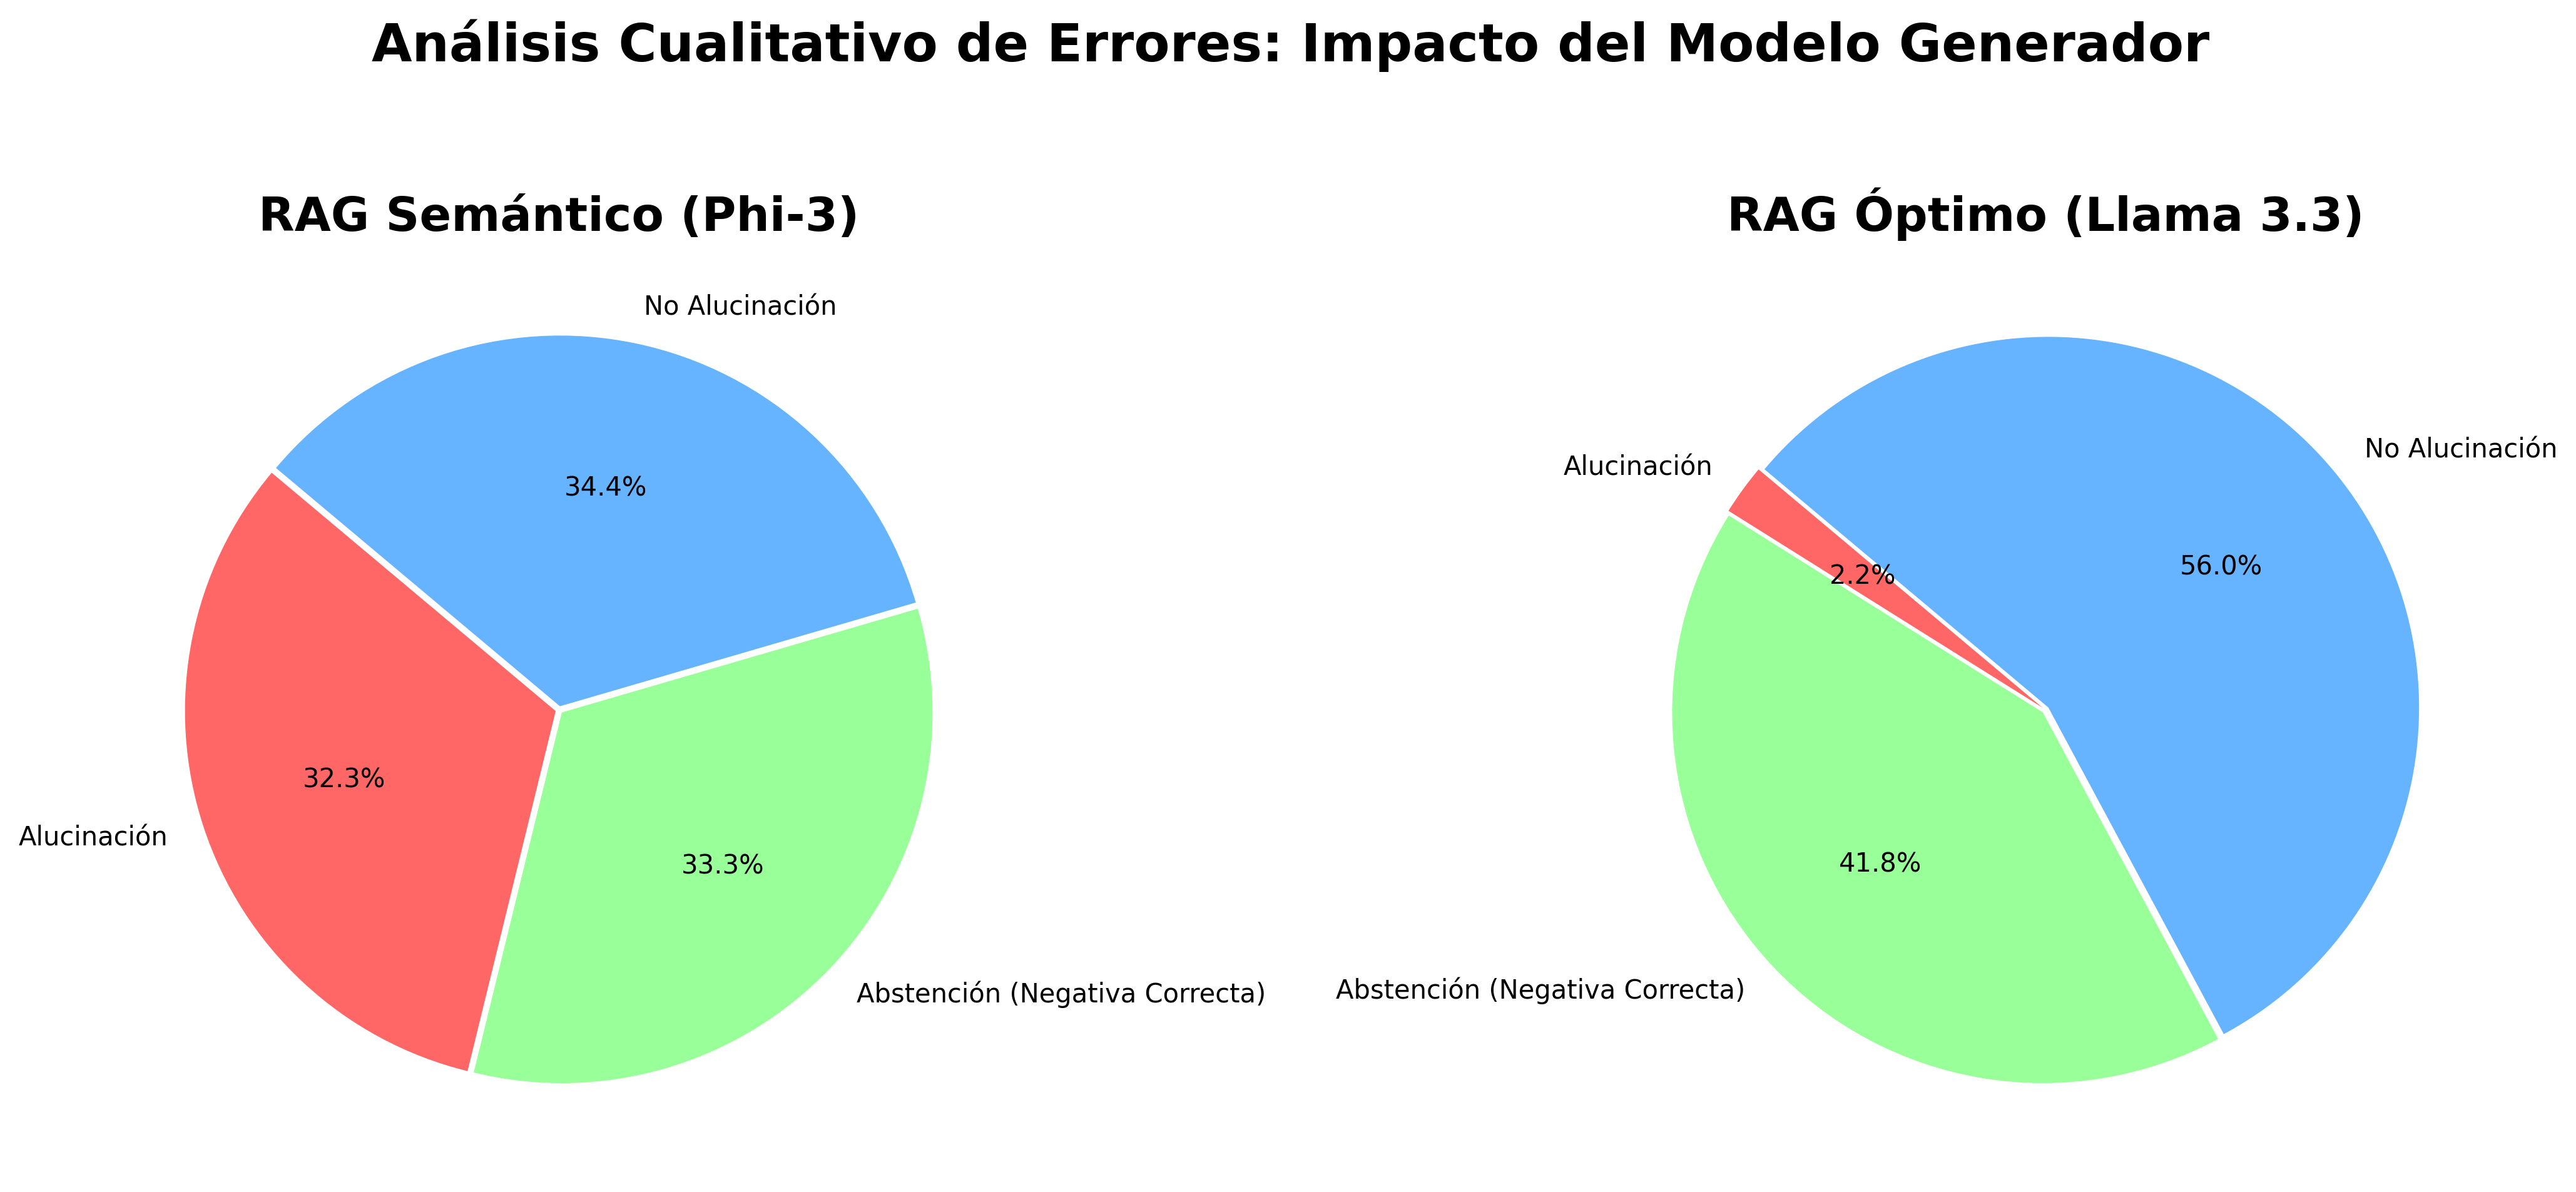
\includegraphics[width=\textwidth]{archivos/grafico_sectores_errores.png}
    \caption{Comparativa cualitativa de errores. Se evidencia la drástica reducción de la tasa de alucinación al emplear un modelo base con mayor grado de alineación.}
    \label{fig:analisis_errores}
\end{figure}

El análisis expuesto en la Figura~\ref{fig:analisis_errores} revela un aspecto fundamental del comportamiento de ambos sistemas. Aunque la diferencia en la tasa de aciertos entre el RAG Semántico con Phi-3 y el RAG Óptimo con Llama 3.3 70B no haya sido super significativa (5\% de aumento), es en la distribución de errores donde se observa un cambio realmente notable. Más allá de acertar un mayor número de preguntas, el verdadero logro de Llama 3.3 70B radica en haber conseguido reducir de forma drástica el porcentaje de alucinaciones ante la falta de información pertinente.

Este comportamiento respalda directamente la premisa detallada en el epígrafe \ref{sec:balance_escala}: Como se observó en la evaluación de los modelos base sin RAG, Llama 3.3 70B ya superaba ampliamente a los otros dos modelos en su capacidad de abstención; esta cualidad intrínseca ha demostrado ser estructuralmente mucho más eficaz al trasladarla a una arquitectura RAG Semántica, mejorando de forma evidente la fiabilidad que teníamos en la mejor arquitectura anterior. Tomando como denominador el total de casos no resueltos correctamente por cada sistema (es decir, excluyendo los aciertos directos), Phi-3 generó alucinaciones en un \textbf{32,3\%} de dichos casos, evidenciando las limitaciones del SLM para seguir instrucciones estrictas. Llama 3.3 70B reduce estos fallos a un \textbf{2,2\%} sobre el mismo denominador.

Al trasladar su superioridad paramétrica al entorno RAG, se observa que Llama 3.3 70B no solo domina las negativas correctas (\textbf{41,8\%}) (vital ya que demuestra la capacidad del sistema para detectar preguntas trampa), sino que altera por completo la naturaleza de los errores que comete. Cuando se enfrenta a una pregunta de la que no logra obtener el contexto adecuado para responder, se abstiene de forma segura en el \textbf{56,0\%} de los casos (\textit{No Alucinación}). En definitiva, el uso de este LLM erradica prácticamente el riesgo de desinformación, transformando las alucinaciones peligrosas en abstenciones y culminando en un marco de \textit{Fact-Checking} mucho más confiable.


	%%%%%%%%%%%%%%%%%%%%%%%%%%%%%%%%%%%%%%%%%%%%%%%%%%%%%%%%%%%%%%%%%%%%%%%%
% Plantilla TFG/TFM
% Universidad de Murcia. Facultad de Informática
% Realizado por: José Manuel Requena Plens
% Modificado: Pablo José Rocamora Zamora
% Contacto: pablojoserocamora@gmail.com
%%%%%%%%%%%%%%%%%%%%%%%%%%%%%%%%%%%%%%%%%%%%%%%%%%%%%%%%%%%%%%%%%%%%%%%%


\chapter{Conclusiones y Vías Futuras}

\section{Conclusiones Generales y Síntesis del Sistema}

El presente Trabajo Fin de Grado partía de una cuestión general expuesta en el capítulo \ref{cap:analisis}: determinar en qué medida una arquitectura RAG permite mitigar las alucinaciones de los modelos de lenguaje y cómo influye la selección de sus componentes en la veracidad final. Tras el análisis de resultados realizado a lo largo del capítulo \ref{cap:diseño}, la conclusión es categórica: la implementación de un sistema de Generación Aumentada por Recuperación no solo mitiga, sino que neutraliza casi por completo la invención de datos, siempre y cuando cumpla dos pilares fundamentales.

El primer pilar radica en la capacidad de extracción de información. La experimentación demostró que navegar eficazmente por un corpus masivo de 490.000 noticias requiere superar las limitaciones de la búsqueda por palabras clave. El uso de un enfoque semántico vectorial (mediante el modelo BGE-M3) superó ampliamente la tasa de acierto del algoritmo léxico tradicional (BM25) en 25.9 puntos porcentuales.

El segundo pilar reside en el tamaño y la calidad del modelo generador. En el ámbito de la verificación de noticias (\textit{Fact-Checking}), el peor escenario posible no es la falta de respuesta ante una consulta, sino la generación de información plausible pero falsa que comprometa la credibilidad del sistema. Bajo esta premisa, la superioridad de Llama 3.3 70B frente al otro modelo evaluado en el RAG (Phi-3) resultó determinante. Al integrar un modelo de gran escala que ya poseía una buena capacidad para abstenerse (52,5\% de acierto en preguntas trampa) sin un \textit{System Prompt} que le diera instrucciones, el sistema RAG óptimo logró transformar casi la totalidad de los fallos de recuperación en abstenciones seguras, reduciendo la tasa de alucinación a un 2,2\% del conjunto de errores cometidos. 

En definitiva, la combinación de una recuperación semántica precisa y un razonamiento robusto conforma una arquitectura altamente fiable. Al indexar el conocimiento en una base de datos vectorial, y confiar la interpretación a un modelo con una buena capacidad de abstención intrínseca, el sistema consigue anular el riesgo elevado de las alucinaciones que poseen otro tipo de sistemas y/o modelos base. Esta investigación confirma que el diseño cuidadoso de arquitecturas RAG representa en la actualidad un estándar seguro para utilizar inteligencia artificial generativa en entornos críticos donde la veracidad es innegociable como es el caso del \textit{Fact-Checking} .

\section{Limitaciones del Sistema y la Metodología}

A pesar de los resultados obtenidos en la configuración final, el sistema desarrollado presenta ciertas limitaciones metodológicas y arquitectónicas que deben ser consideradas:

\begin{itemize}
    \item \textbf{Limitaciones computacionales y de infraestructura:} El procesamiento masivo de información y la evaluación del \textit{dataset} conllevaron tiempos de ejecución relativamente elevados. Además, la dependencia de APIs para acceder a modelos mas potentes introdujo restricciones por límites de cuota y peticiones simultáneas (\textit{rate limits}). Asimismo, estas restricciones condicionaron la selección de los modelos evaluados; si bien Llama 3.3 70B ofreció un rendimiento excepcional, el estudio no incluyó el uso de modelos comerciales que son mucho más avanzados (como las últimas versiones de la familia GPT, Gemini o Claude) debido a los costes asociados a su uso.

    \item \textbf{El marco de evaluación automática (\textit{LLM-as-a-Judge}):} La implementación de un modelo de parámetros masivos (120B) como juez automatizado resultó ser una herramienta excelente para procesar eficientemente la batería de preguntas y acelerar el proceso de corrección. Sin embargo, delegar la verificación en otra inteligencia artificial introduce el riesgo de heredar sesgos interpretativos del modelo evaluador, pudiendo ocasionar errores de corrección. Dado que el sistema automatizado no es infalible, la metodología requirió de la integración de una capa de supervisión humana (una lectura rápida de verificación) para revisar principalemente las preguntas de inferencia y garantizar la precisión absoluta de las métricas presentadas, impidiendo una autonomía total del proceso de corrección.

    \item \textbf{Corpus estático y temporalidad:} El marco operativo del sistema está estrictamente restringido a la base de datos indexada, compuesta por aproximadamente 490.000 noticias preprocesadas. Al tratarse de un corpus estático y carecer de conexión a internet en tiempo real, la arquitectura es incapaz de recuperar información o verificar afirmaciones sobre eventos recientes que hayan ocurrido con posterioridad a la extracción de los datos. Por consiguiente, la efectividad del sistema está sujeta a una ventana temporal cerrada, limitando su aplicabilidad inmediata como herramienta de validación de noticias de última hora en un entorno periodístico real.
\end{itemize}

\section{Consideraciones Éticas en la Detección de Desinformación}

El desarrollo e implementación de sistemas automatizados para tareas de \textit{Fact-Checking} conlleva implicaciones éticas profundas que trascienden la dimensión puramente técnica. Un sistema diseñado para dictaminar qué constituye una "verdad" o una "mentira" asume una gran responsabilidad, ya que sus veredictos pueden influir significativamente en la percepción de los usuarios. En este contexto, el mayor riesgo reside en la posibilidad de que el usuario final desarrolle una confianza ciega en la herramienta, delegando su juicio crítico en la Inteligencia Artificial.

Es fundamental subrayar que el éxito arquitectónico de un sistema RAG se basa en asumir que los documentos recuperados contienen la verdad absoluta; sin embargo, el hecho de que una afirmación aparezca publicada en un medio de comunicación no garantiza su veracidad irrefutable. Los corpus de noticias, por su propia naturaleza periodística y editorial, son susceptibles de contener sesgos. 

En este sentido, el impacto de dichos sesgos varía drásticamente según el tipo de consulta. Por un lado, en las \textbf{preguntas factuales} (fechas, nombres, datos concretos), el riesgo de sesgo es menor; si la recuperación es correcta, el sistema solo fallaría si la noticia original fuera directamente falsa o contuviera un error tipográfico (un fenómeno evidenciado en el Caso 5 del epígrafe 4.3.1, donde el sistema reprodujo un error de redacción de la fuente periodística alterando la fecha de fundación de una empresa). Por otro lado, en las \textbf{preguntas de inferencia}, el riesgo se multiplica exponencialmente, ya que aunque los hechos base de la noticia sean reales, el texto puede estar redactado con un enfoque o intencionalidad particular, lo cual hace que el sistema corra el riesgo de heredar y amplificar el sesgo editorial de la fuente, presentándolo al usuario como un razonamiento puramente objetivo.

Por consiguiente, este sistema RAG no debe concebirse en ningún caso como un sistema de juicio absoluto. Su propósito ético e ideal es ser una ayuda para periodistas, verificadores humanos y usuarios críticos a la hora de verificar información, proporcionando un marco rápido de contraste de información que siempre debe estar sujeto a la revisión y validación final humana.

\section{Vías Futuras}

Si bien el sistema propuesto ha establecido una base robusta y competitiva para la mitigación de alucinaciones en tareas de verificación, la rápida evolución del ecosistema de la Inteligencia Artificial abre diversas líneas de investigación para perfeccionar y expandir la arquitectura en trabajos futuros. He decidido seleccionar tres vías de desarrollo:

\begin{itemize}
    \item \textbf{Evolución hacia un RAG Dinámico (Agentic RAG):} Para superar la limitación temporal del corpus estático actual, el siguiente paso consistiría en dotar al sistema de acceso a internet en tiempo real. Mediante el uso de herramientas de búsqueda web (\textit{Web Search}) o arquitecturas de agentes, el recuperador podría indexar noticias publicadas en el momento de la consulta. Esto permitiría al sistema contrastar eventos de última hora y desinformación emergente, multiplicando su utilidad práctica.

    \item \textbf{Modelos de Frontera frente a Optimización Local (\textit{Fine-Tuning}):} Para intentar reducir el 2,2\% de error crítico actual al cero absoluto, resultaría de gran interés evaluar el impacto de integrar APIs comerciales mucho más avanzadas. Como contraparte a este enfoque de alto coste, una vía de investigación sumamente valiosa consistiría en aplicar técnicas de ajuste fino (\textit{fine-tuning}) sobre modelos locales ligeros, como el propio Phi-3. El objetivo sería entrenarlo específicamente para adquirir el comportamiento de abstención ("No lo sé") que Llama 3.3 70B demostró tener de forma natural, logrando así un sistema de alta fiabilidad computacionalmente muy económico.

    \item \textbf{Integración de Multimodalidad:} En el ámbito actual de las \textit{Fake News}, gran parte de la desinformación no se difunde exclusivamente mediante texto, sino a través de fotografías manipuladas o descontextualizadas. Una evolución clave del sistema pasaría por incorporar modelos de visión artificial capaces de procesar una imagen de entrada, extraer su contexto semántico y cruzarlo con la base de datos periodística para verificar si la imagen corresponde a los hechos relatados.
\end{itemize}
	%%%%
	% CONTENIDO. BIBLIOGRAFÍA.
	%%%%
	\nocite{anthropic2026claude, google2026gemini}
	\bibliographystyle{unsrtnat}
	\bibliography{bibliografia/bibliografia} % Archivo que contiene la bibliografía
	
	
	%%%%
	% CONTENIDO. LISTA DE ACRÓNIMOS. Comenta las líneas si no lo deseas incluir.
	%%%%
	% Incluye el listado de acrónimos utilizados en el trabajo. 
	\printglossary[style=modsuper,type=\acronymtype,title={Lista de Acrónimos y Abreviaturas}]
	% Añade el resto de acrónimos si así se desea. Si no elimina el comando siguiente
	\glsaddallunused
	
	%%%%
	% CONTENIDO. Anexos - Añade o elimina según tus necesidades
	%%%%
	\appendix % Inicio de los apéndices
	
\end{document}